\subsection{Collect comparable data}

Currently, there are three available datasets (matrices): zoobenthic community data (311 by 16),
chemical data (104 by 30), and environmental data (289 by 7).
These matrices can be merged by the station ID, which gives a comparable dataset with 104 rows
and 53 columns. 

\begin{figure}[!h]
    \centering
    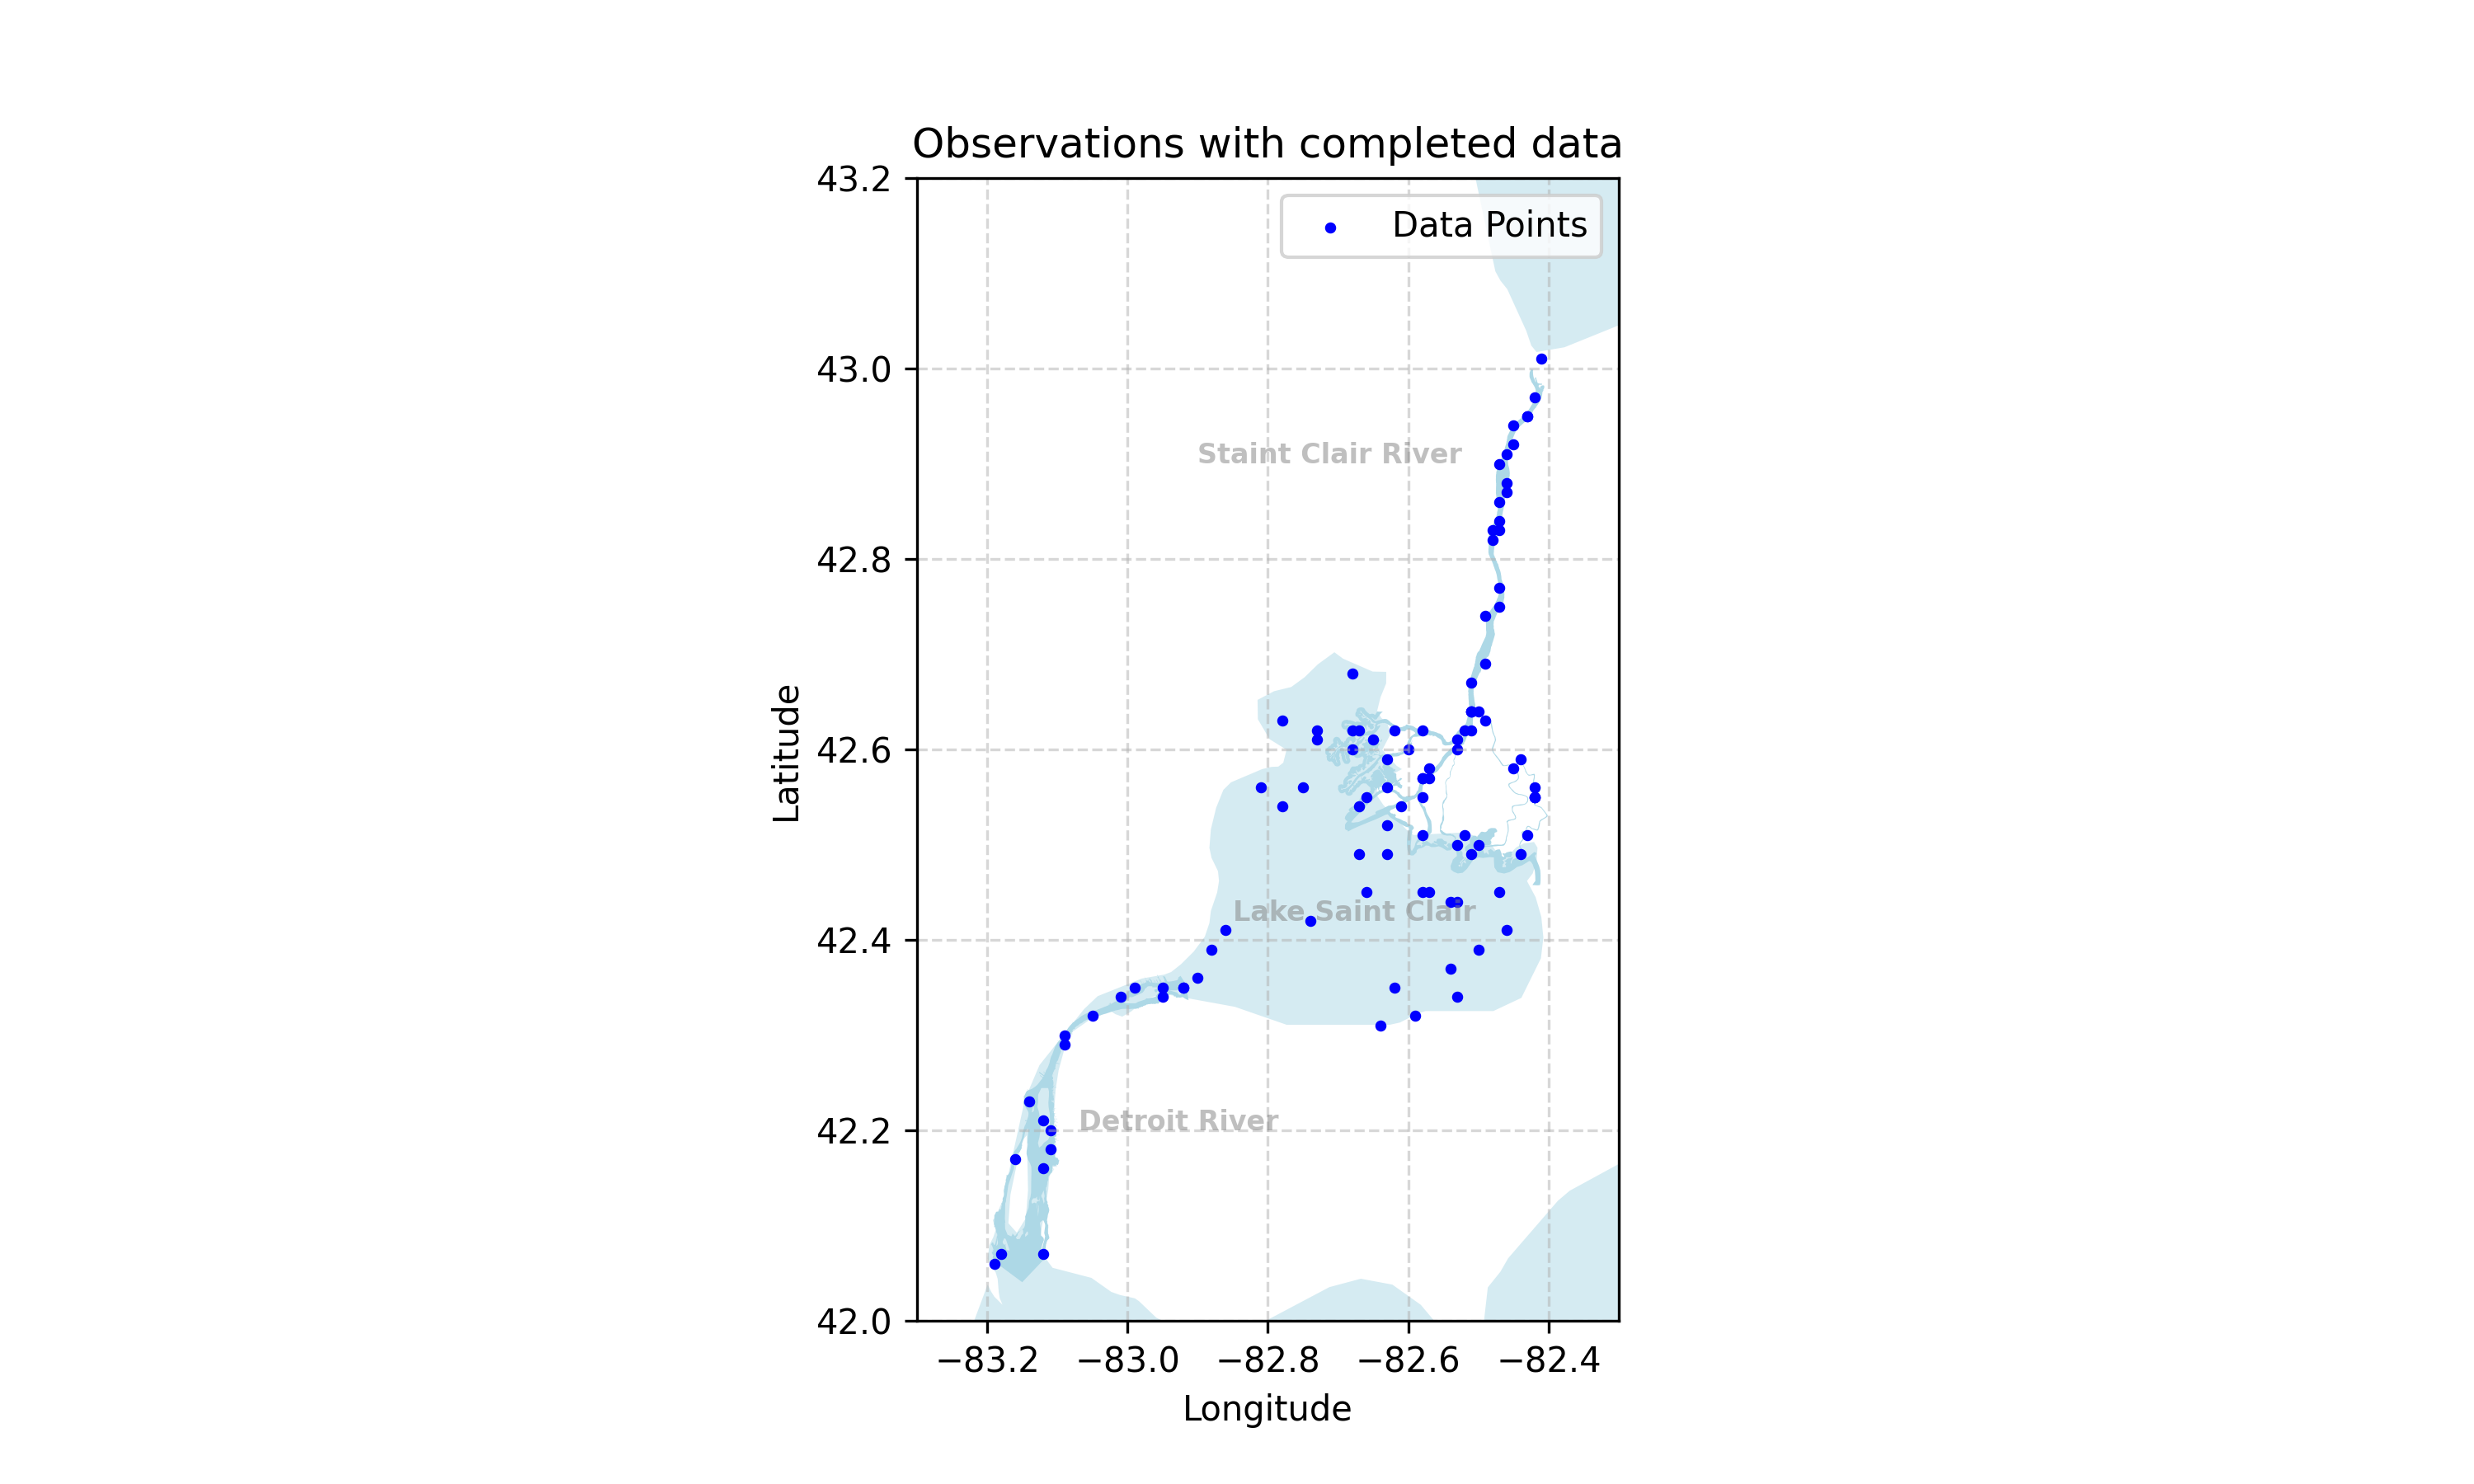
\includegraphics[width=\textwidth]{../results/preliminary_results/merged_104_completed_observations.png}
    \caption{Distribution of the 104 sites with completed three types of data.}
    \label{fig:merged_104_completed_observations}
\end{figure}

Figure \textcolor{blue}{\ref{fig:merged_104_completed_observations}} shows the distribution of the 104 sites
with completed three types of data, these observations are generally evenly distributed
across the Huron-Erie Corridor, which backs up the belief in sampling aspect that the top \(p\%\) sites
in stress level should have no or minimal human disturbances.

\subsection{Assess sediment contamination and Identify reference and degraded sites}

In this stage, log-transformation was applied on the chemical data to 
reduce the dominance of some chemical variables that have large values. 
Then, PCA was applied on the transformed chemical data 
and the distribution of loadings across the chemical variables
were computed for each principal component for the upcoming selecting PCs step.

\begin{figure}[!h]
\centering
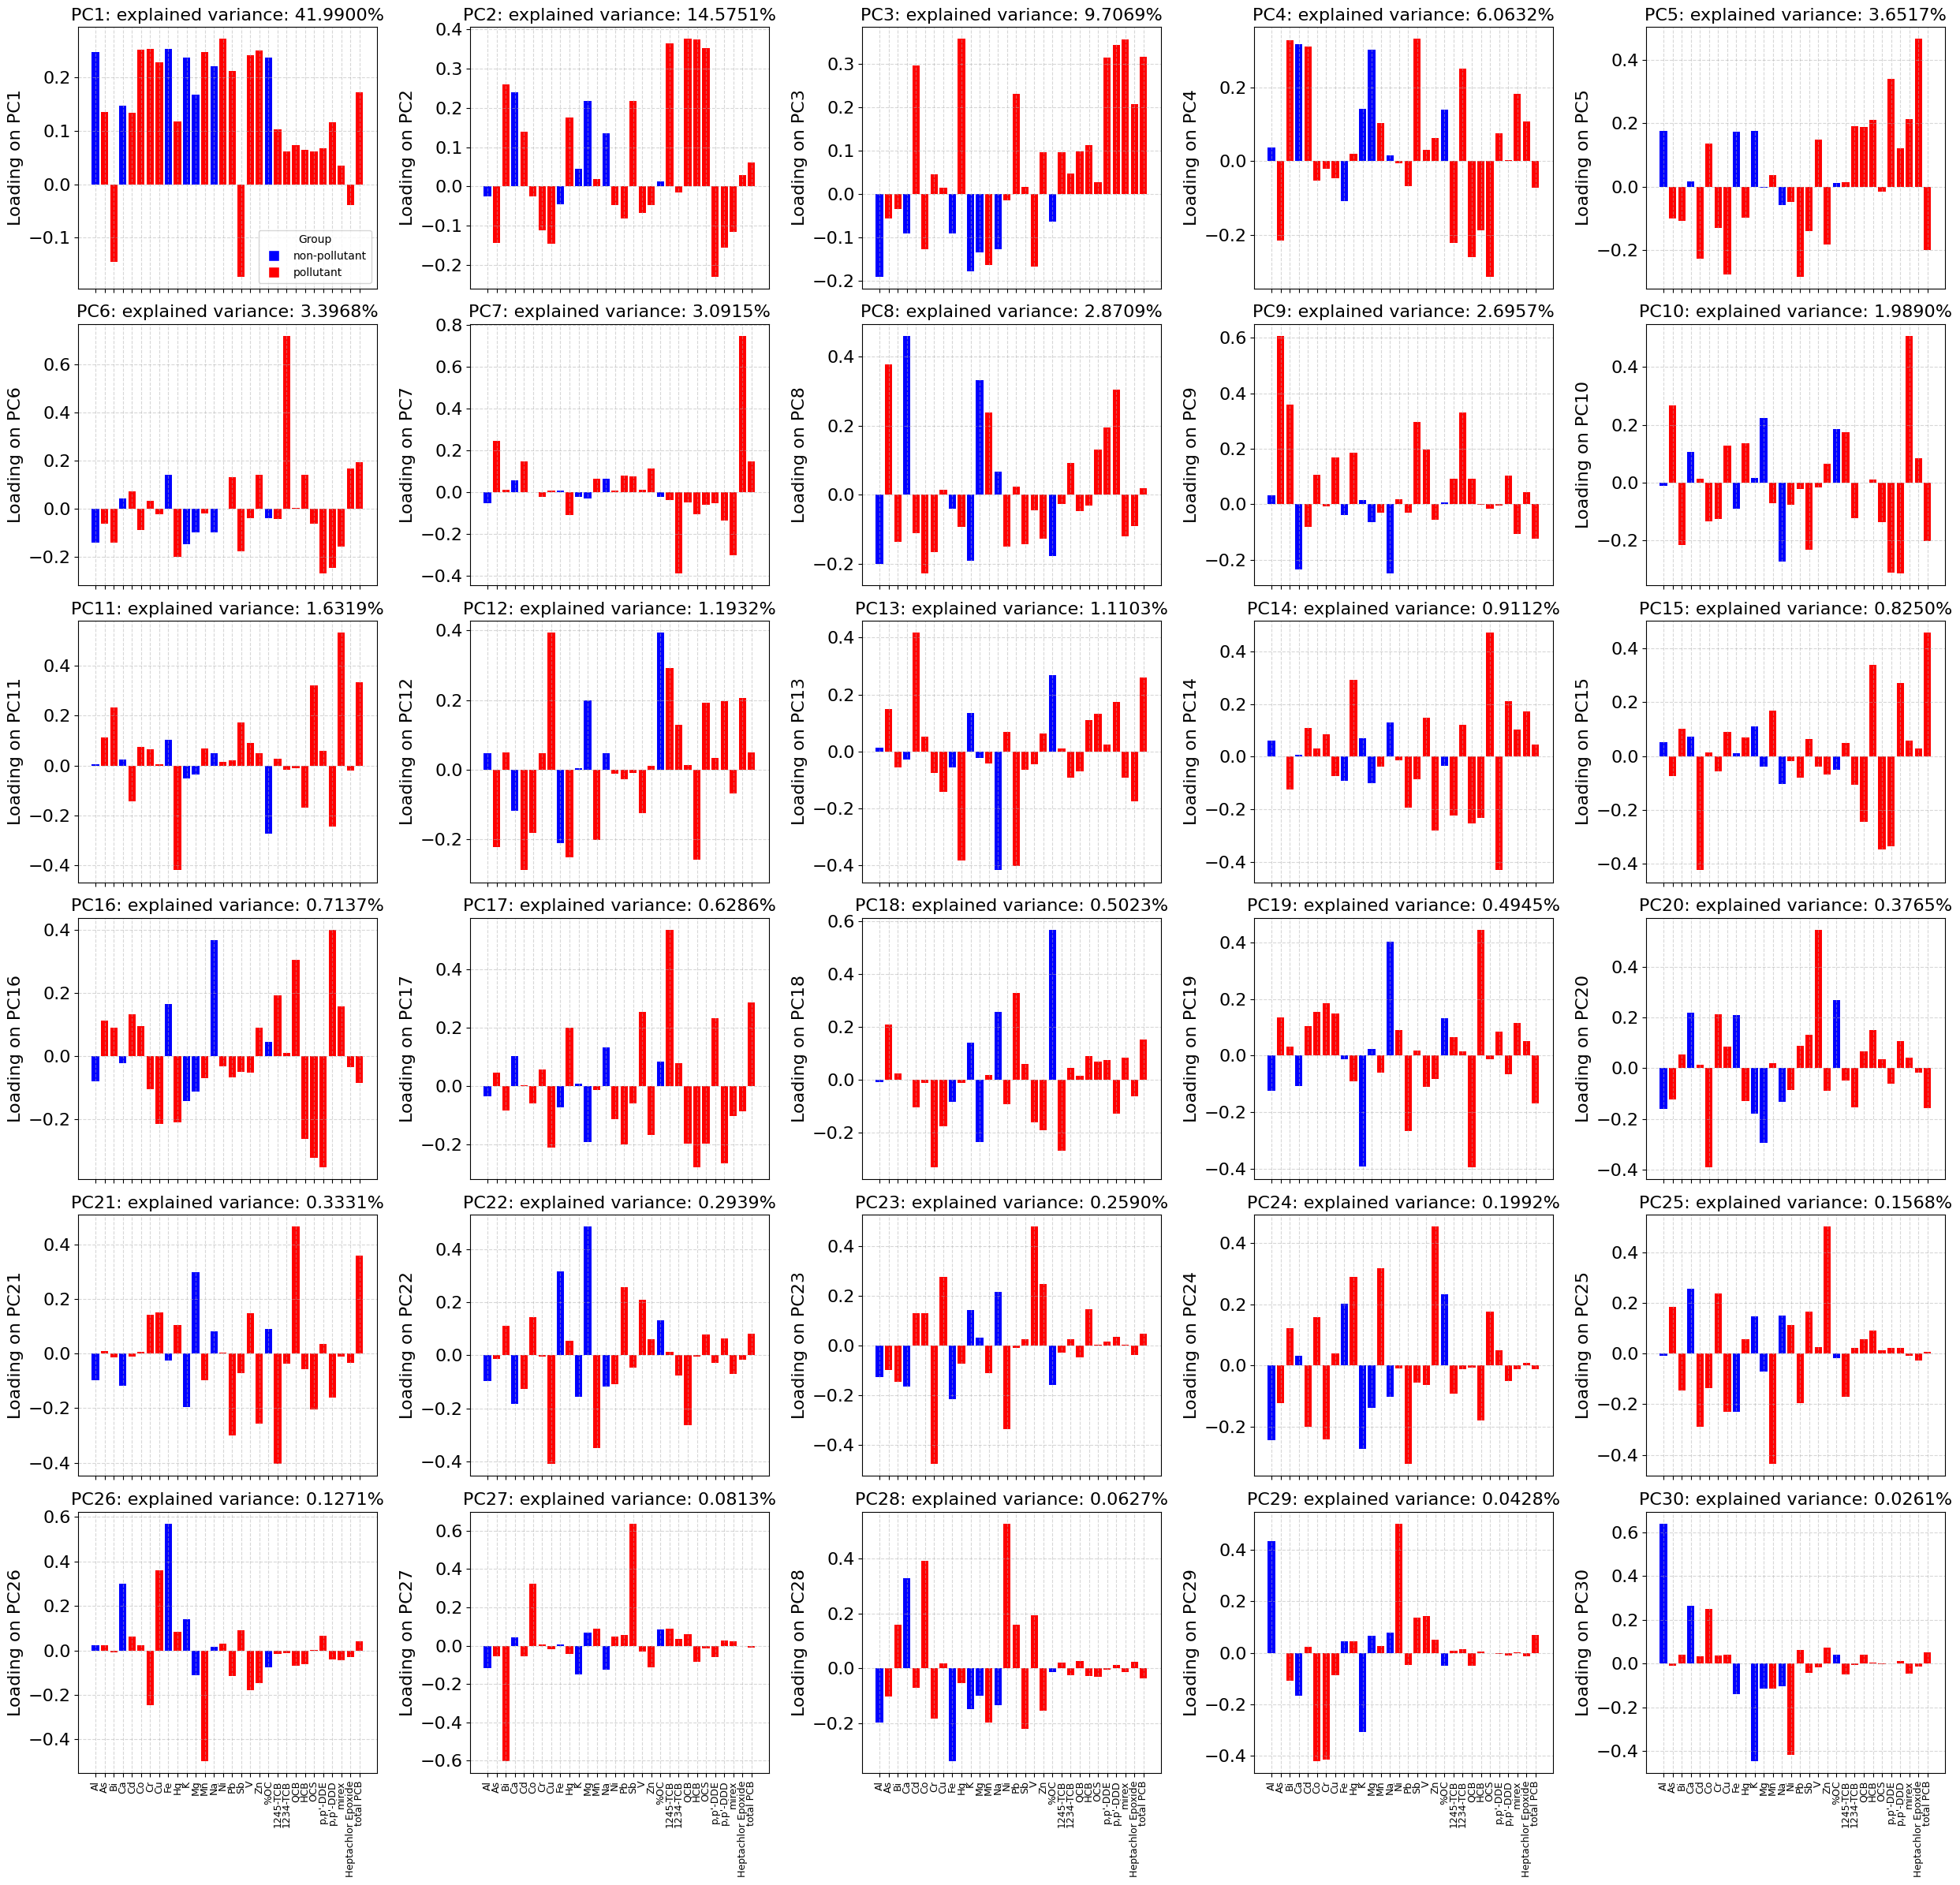
\includegraphics[width=\textwidth]{../results/preliminary_results/pca_loadings_chemical_updated.png}
\caption{PCA loadings of the chemical data, showing the distribution of loadings across chemical variables}
\label{fig:pca_loadings_chemical_updated}
\end{figure}

Not all PCs are used to compute the stress score, there are three criteria to select the suitable PCs:

\begin{itemize}
    \item Selected PCs should have a relatively high proportion of variance explained(high eigenvalue).
    \item Selected PCs should have a high loading on the chemical variables that are pollutants and rarely sourced from nature.
    \item Selected PCs should avoid the counteracting effect due to uniform distributed positive and negative loadings
    across the chemical variables.
\end{itemize}

After applying the above criteria, 'PC1', 'PC2', 'PC3', 'PC5', 'PC6', 'PC7', 'PC9' are selected as the suitable PCs.

Based on the selected PCs, these PCs were normalized to the range [0, 1] to eliminate the effect of differing scales
(due to their eigenvalues), reflecting the real-world situation that the toxicity of chemical elements is
not directly comparable and not always proportional to their concentrations. Subsequently,
the normalized PCs were summed, considering the directionality of positive and negative loadings,
to obtain the "SumReal" score\footnote{As done by Jian in her sediment contamination assessment}, 
for each sample, which serves as a measure of sediment contamination.

After this step, each observation in the dataset has a "stress score" ("SumReal" score, as Jian defined in her thesis),
the lower the score, the more contaminated the sediment is.

Based on the "SumReal" score, reference and degraded sites were identified by selecting
the lowest 20\% and highest 20\% of the "stress score", respectively.
There selected reference sites will be viewed as minimally disturbed sites, and 
their taxa compositions will be thought as determined completely by the environmental factors.


These references support building a purely tidy model that predicts what
a pristine taxa composition should be given a specific set of environmental conditions
(if the distribution of the
environmental factors is uniform across all possible values or fit to the real world distribution).

\begin{figure}[!h]
    \centering
    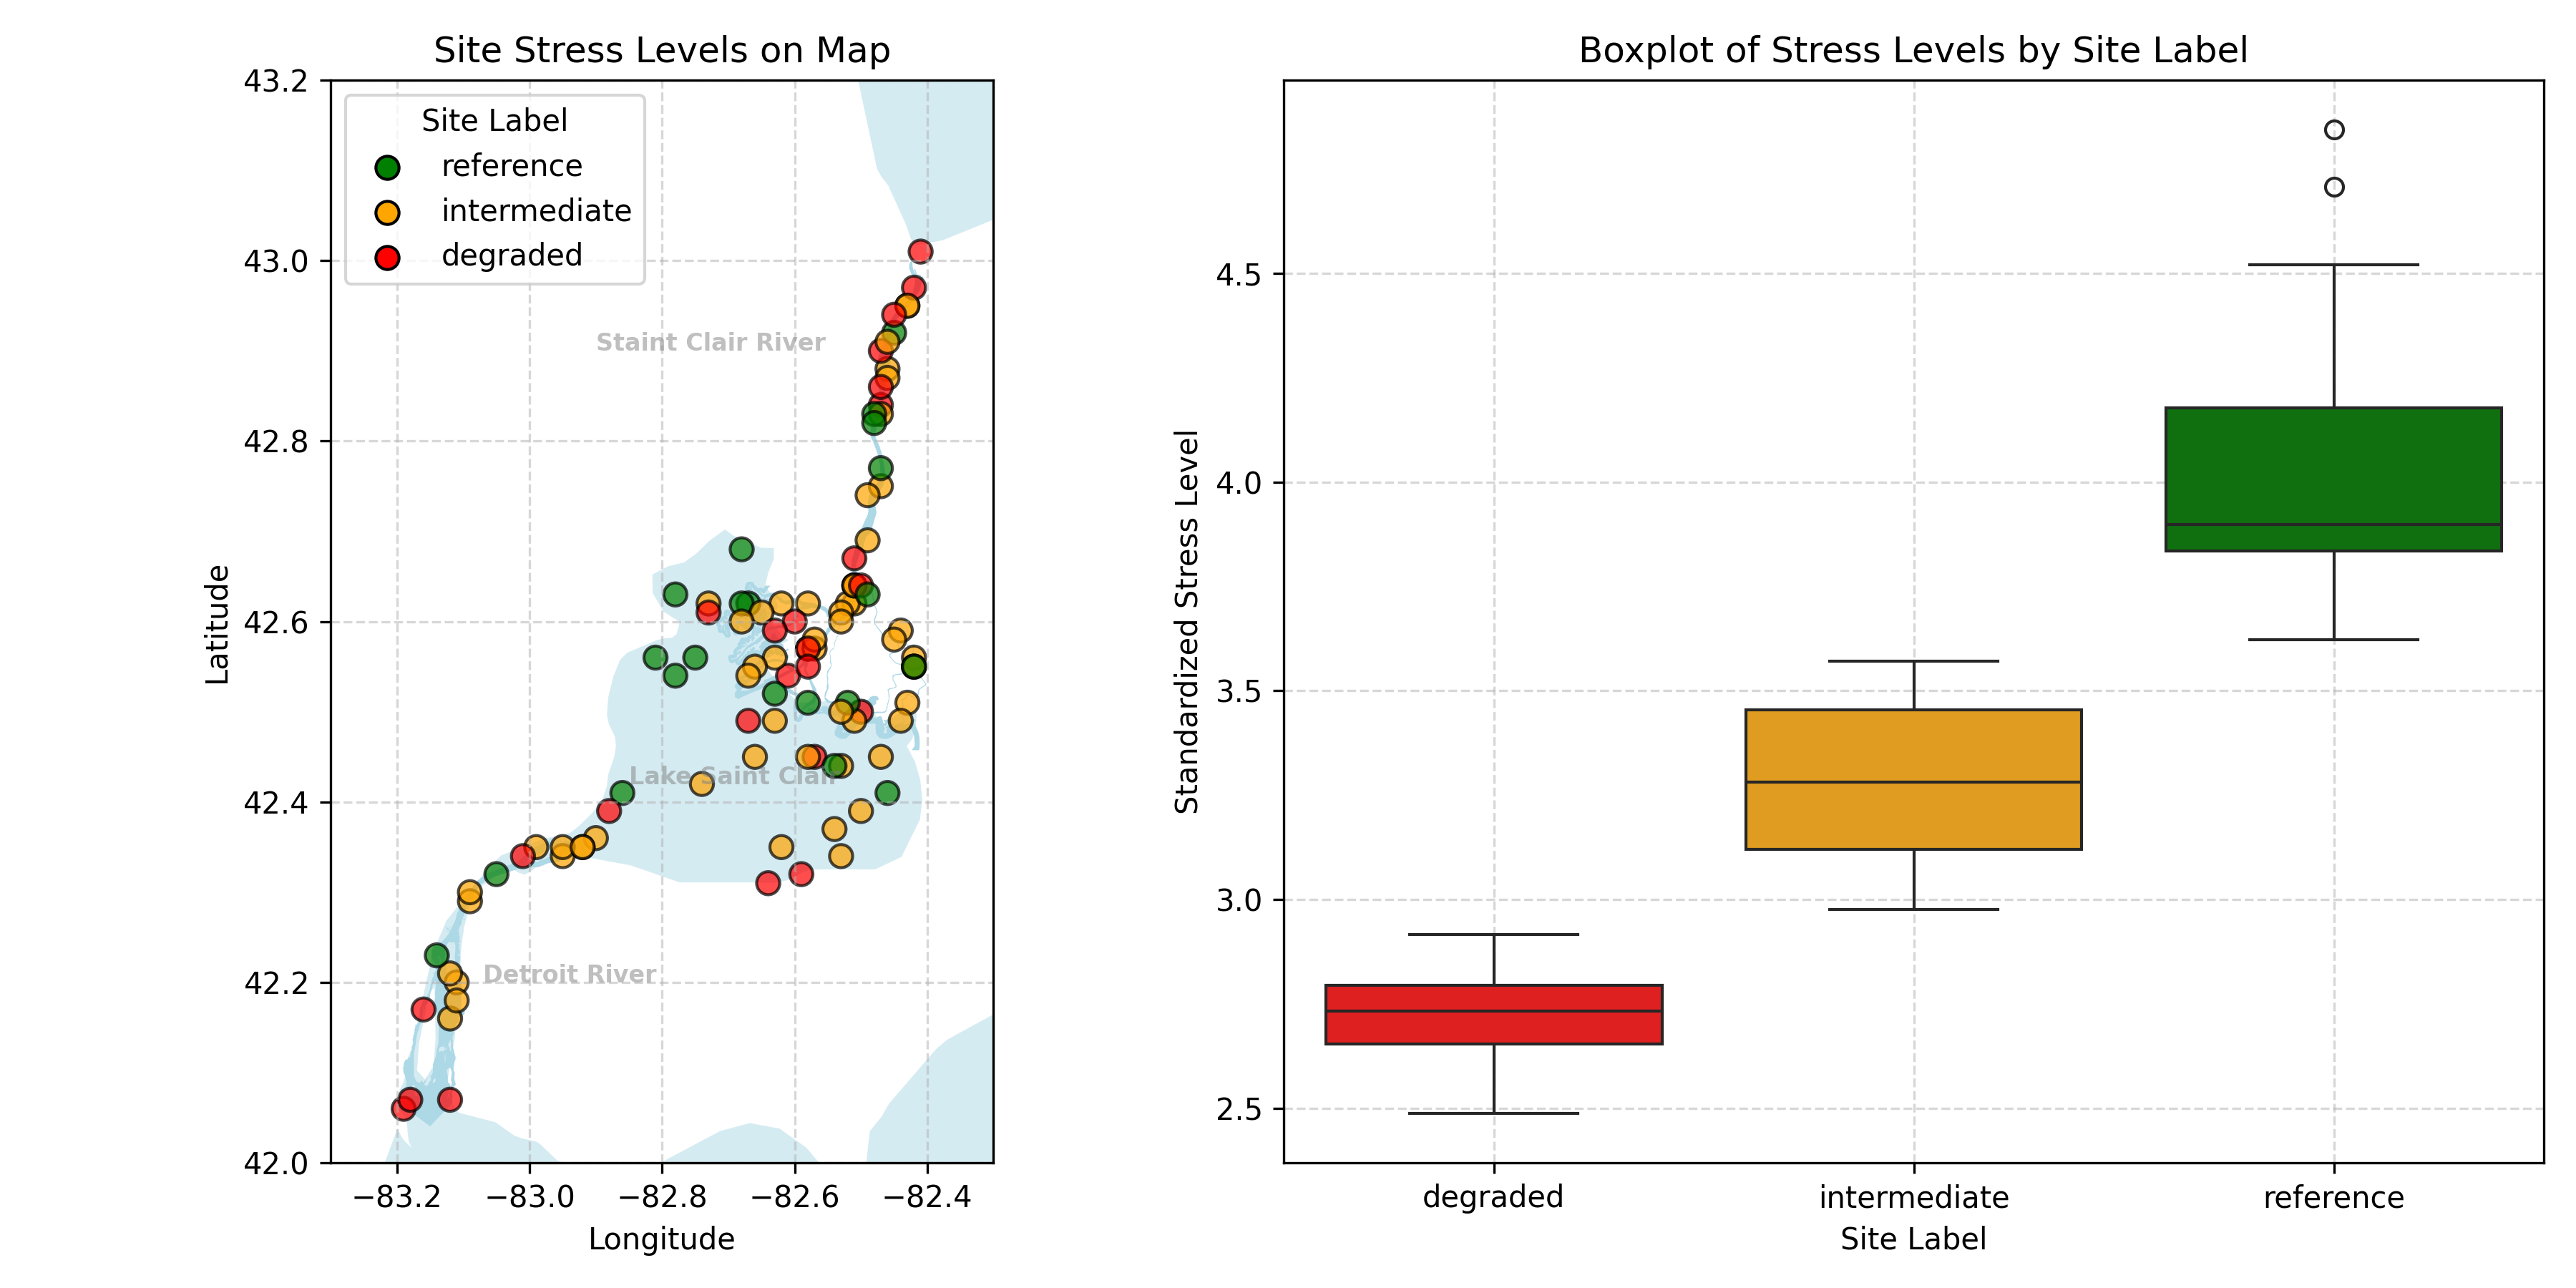
\includegraphics[width=\textwidth]{../results/preliminary_results/stress_levels_map_and_boxplot.png}
    \caption{Map and boxplot of stress levels across three blocks of stress levels: 
    reference(top 20\% of stress scores), degraded(bottom 20\% of stress scores) and others}
    \label{fig:stress_levels_map_and_boxplot}
\end{figure}

\begin{figure}[!h]
    \centering
    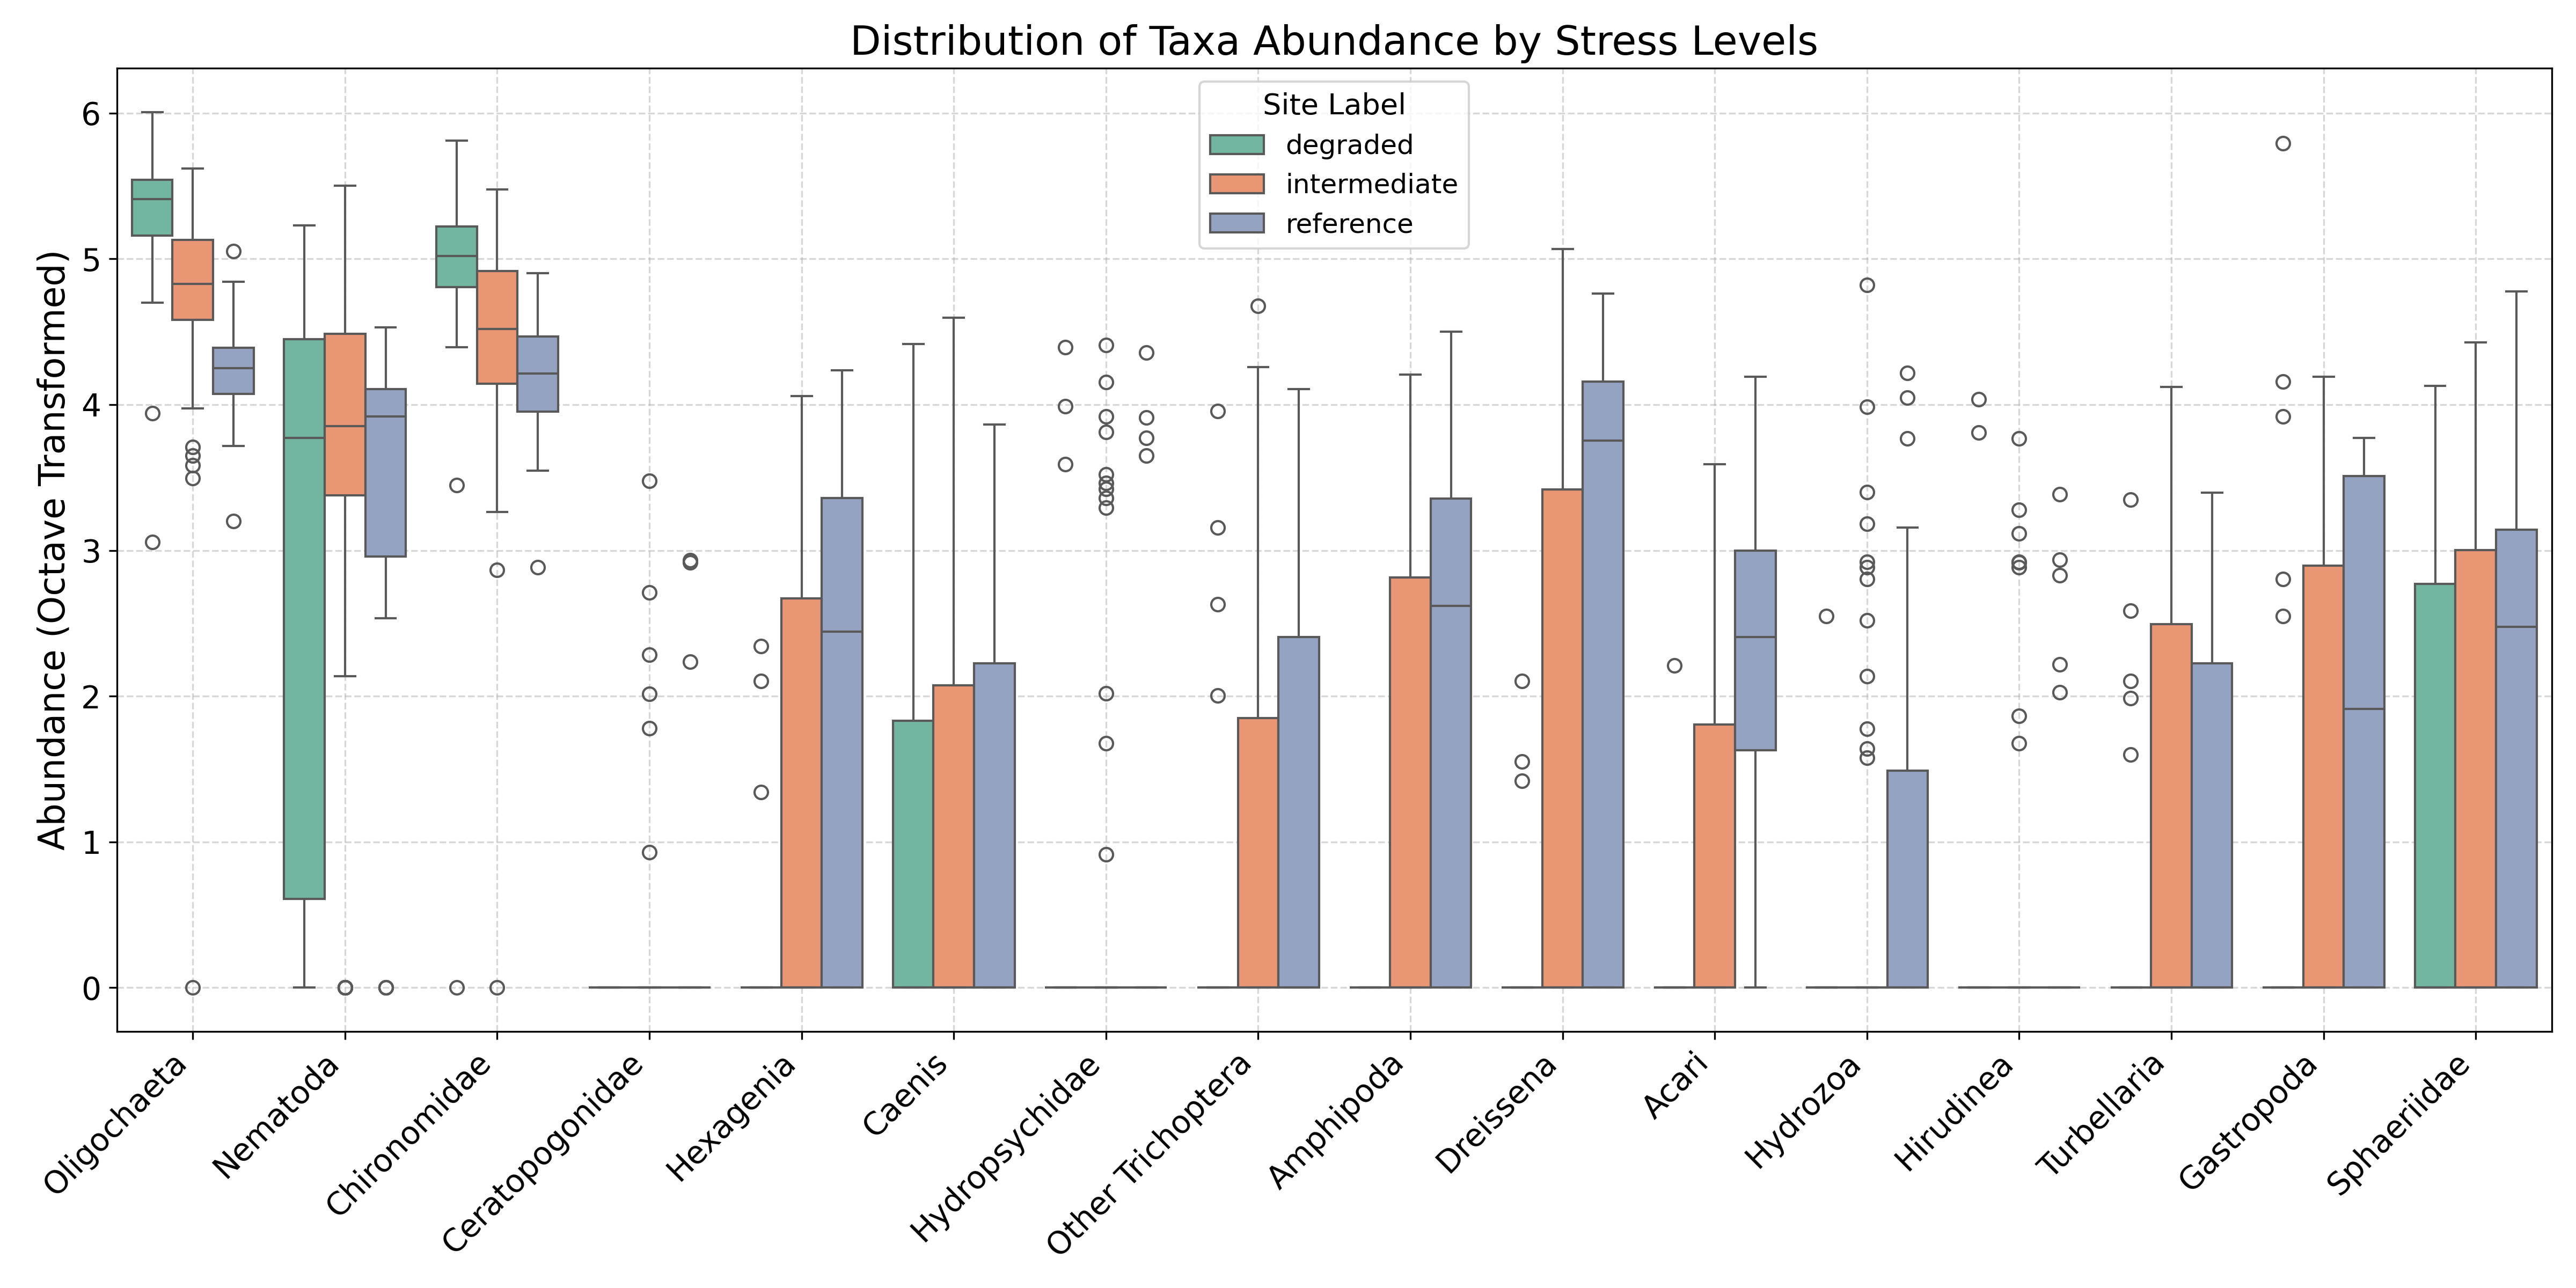
\includegraphics[width=\textwidth]{../results/preliminary_results/taxa_abundance_by_site_label.png}
    \caption{Taxa abundance distribution by site label, 
    showing the potential taxa composition differences 
    across three blocks of sediment contamination}
    \label{fig:taxa_abundance_by_site_label}
\end{figure}

Figure \textcolor{blue}{\ref{fig:taxa_abundance_by_site_label}} shows the box plots of taxa abundance across the three blocks.
Even though it is not accurate to know the taxa composition across stress levels,
but a good result is that the taxa abundance distribution is different across the types: degraded, intermediate and reference.
Because such blocking operation controls the human disturbances to some extent, and
we hope to see the taxa composition differences across these disturbance levels.
Although Figure \textcolor{blue}{\ref{fig:taxa_abundance_by_site_label}} might not provide a complete and satisfying 
picture, but it is acceptable considering that we have not controlled the environmental factors yet.

\clearpage
\subsection{Cluster reference sites by taxa community composition}

In this step,  IQR method was applied to detect outliers in the taxa data, 
and octave transformation was applied as suggested in Jian's analysis,
to reduce the impact of outliers and balance the influence of all taxa.

The octave transformation is applied by the following formula, where the proportion of a taxon 
at a site is the proportion of the taxon in the total density of all taxa at the site.

\[
x_\text{octave transformed} = \log_2(100 \times (\text{proportion of taxa}  + 0.01))
\]

After the transformation, there were less outliers and flatter distribution of the taxa data.

\begin{figure}[!h]
    \centering
    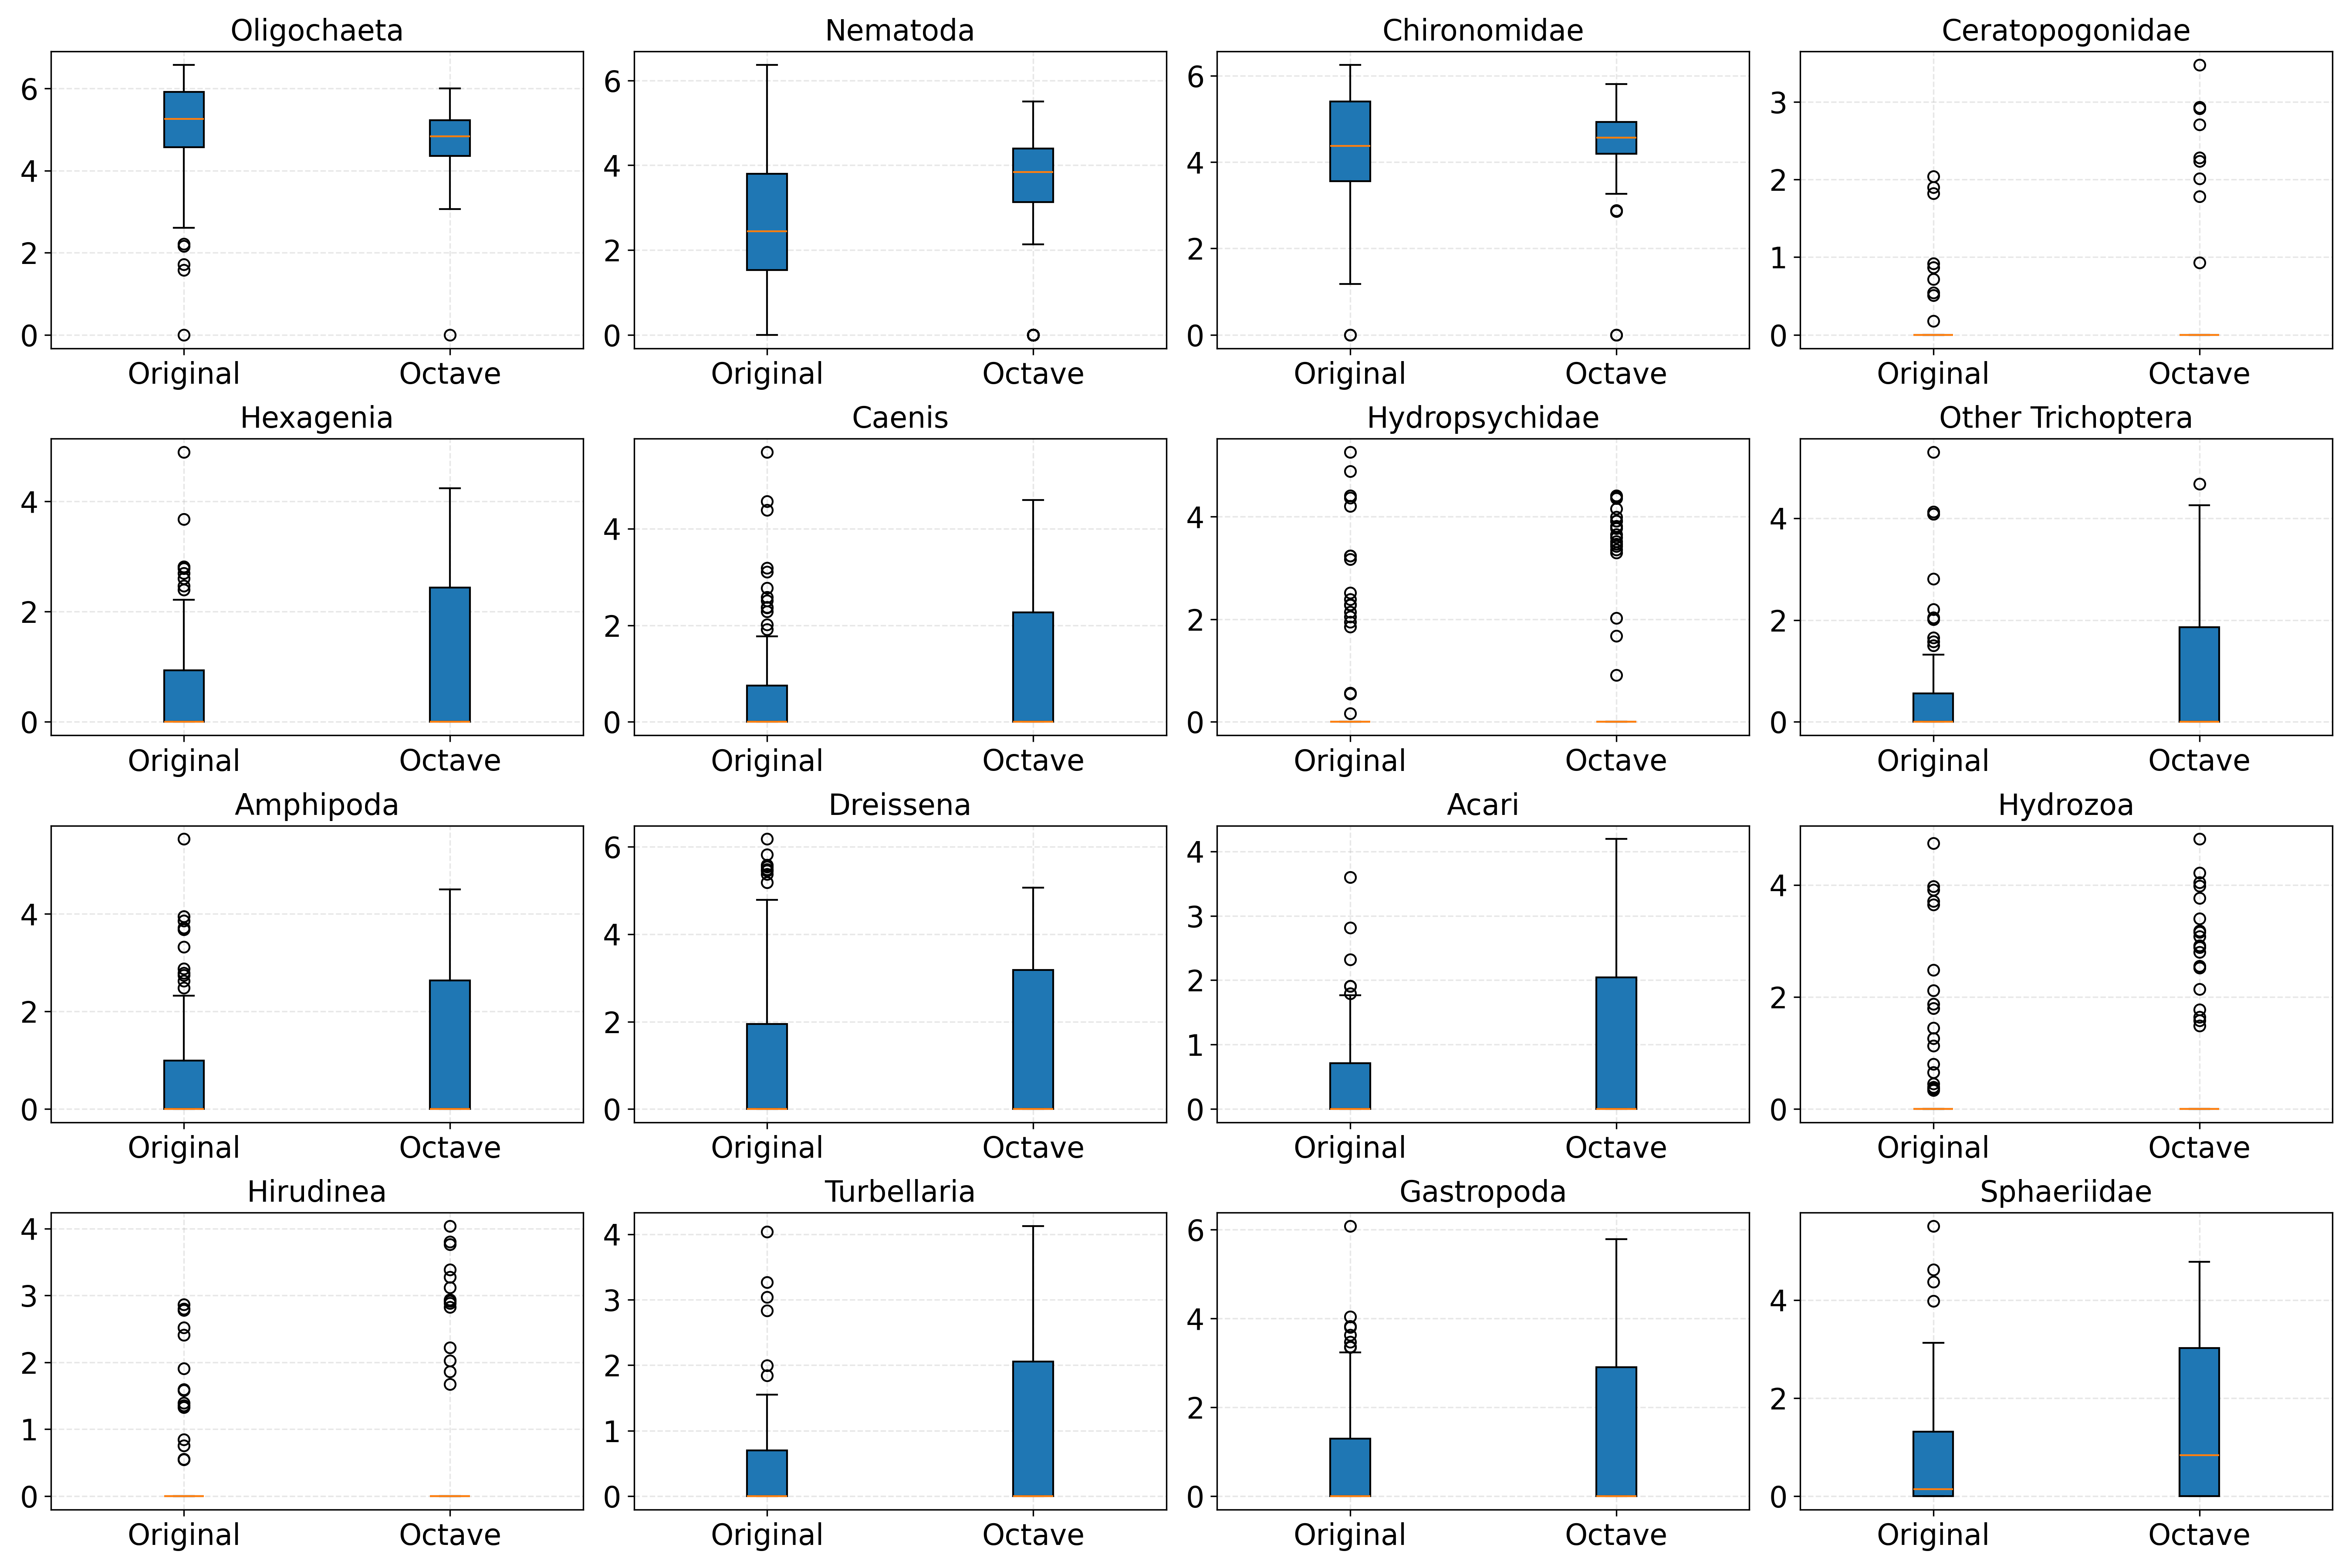
\includegraphics[width=\textwidth]{../results/preliminary_results/octave_transformed_taxa_boxplots.png}
    \caption{Boxplots of the original vs octave-transformed taxa data, showing reduced outliers and more balanced distribution.}
    \label{fig:octave_transformed_taxa_boxplots}
\end{figure}

Based on the octave-transformed taxa data, clustering was applied to identify major taxa community patterns across different environmental conditions.
The clustering was performed using hierarchical clustering method, and the number of clusters \(K\) was set to 3 based on the dendrogram analysis.

\begin{figure}[!h]
    \centering
    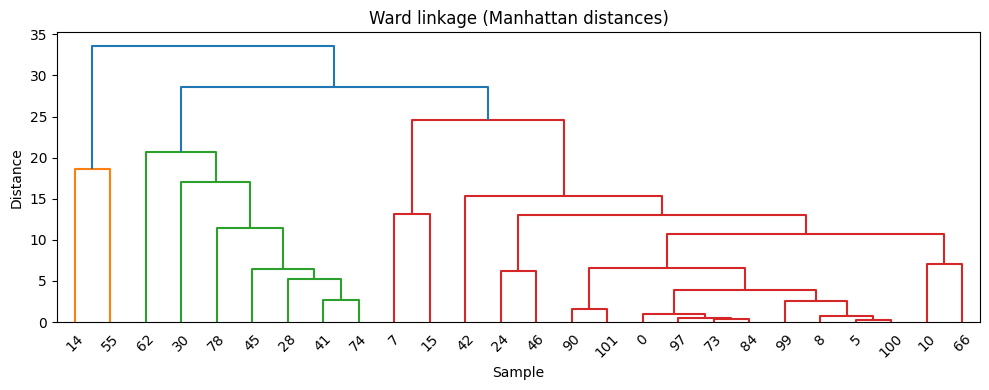
\includegraphics[width=\textwidth]{../results/preliminary_results/clustering_on_references_taxa.png}
    \caption{A possible example of clustering results of reference sites by taxa composition, showing the major groups of minimally disturbed taxa compositions.}
    \label{fig:clustering_on_references_taxa}
\end{figure}

Figure \textcolor{blue}{\ref{fig:clustering_on_references_taxa}} is an example of the clustering results on references, 
and it is not the final clustering result. It was noticeable that one cluster (orange color) has only 2 reference sites in 
it, which is not enough to represent a stable "ideal" taxa composition and to fit a discriminant function for its cluster.

Considering it is in the preliminary stage, this example is presented here only for showing
the clustering process and the potential taxa community patterns across different environmental conditions.
A better clustering result needs to include enough reference sites in each cluster for constructing a stable 
"ideal" taxa composition benchmark and to support the upcoming fitting of a discriminant function, \(f_{k, \tau}(z)\).
However, the sampled environmental conditions are also important to be considered, a uniform sample-environment distribution 
or a proportional to the real world distribution is better for the clustering to be meaningful.

\begin{figure}[!h]
    \centering
    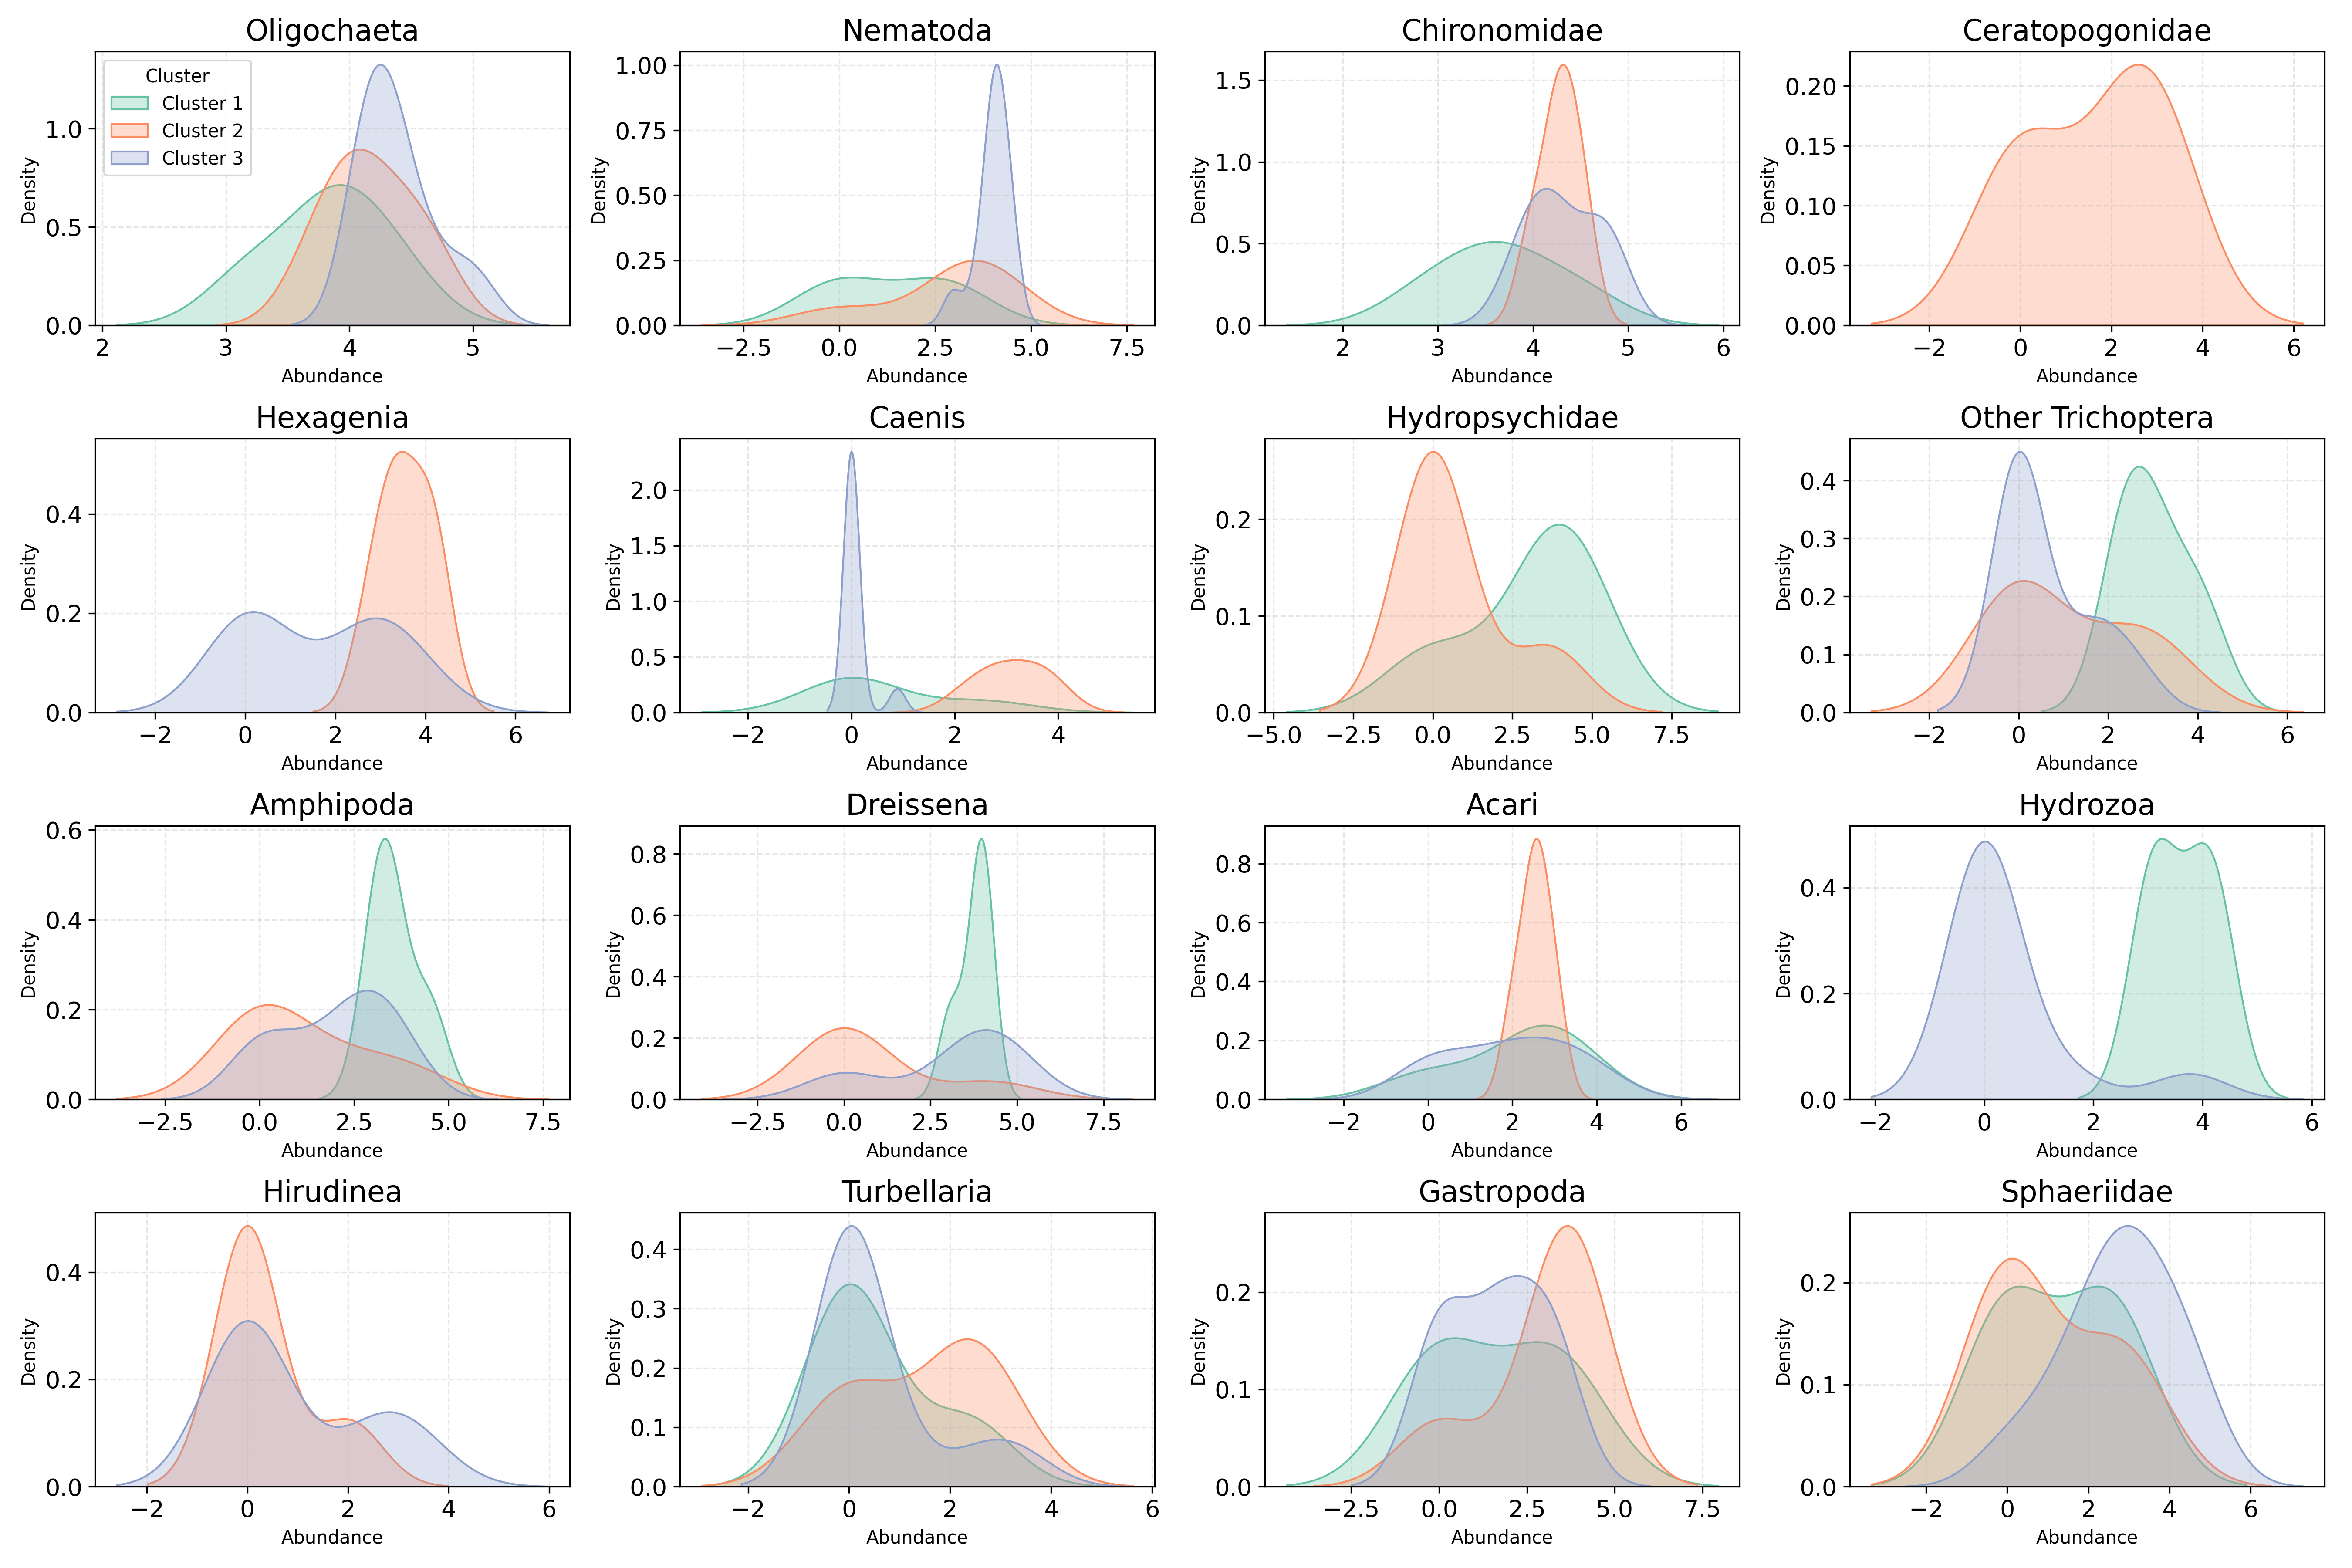
\includegraphics[width=\textwidth]{../results/preliminary_results/taxa_density_by_cluster.png}
    \caption{"Ideal" individual taxa density across clusters, showing the distribution of taxa across different clusters of reference sites.
    (The disappearance of the density curve of some taxa in a cluster means that the taxa is not present in the cluster.)}
    \label{fig:taxa_density_by_cluster}
\end{figure}

Figure \textcolor{blue}{\ref{fig:taxa_density_by_cluster}} shows the taxa density distribution across clusters.
The sites in each cluster are both controlled by the environmental conditions(clustering results)
and the human disturbances(reference sites, no or minimal human disturbances), 
so we hope to see their taxa community compositions(density curves) difference across 
the current clusters.

\subsection{Fit Discriminant Function of environmental factors for taxa clusters}

At this stage, a discriminant function(classifier) was fitted on these reference sites to 
predict cluster memberships(labels) with their environmental factors.
Table \textcolor{blue}{\ref{tab:lda_coeffs}} shows the coefficients of the fitted discriminant function,
and Table \textcolor{blue}{\ref{tab:lda_report}} shows the classification report of the fitted discriminant function
on the training set of reference sites.

\begin{table}[!h]
\centering
\caption{Discriminant Coefficients}
\label{tab:lda_coeffs}
\begin{tabular}{>{\centering\arraybackslash}m{3.5cm}*{3}{>{\centering\arraybackslash}m{2.5cm}}}
\toprule
 & $Class_1$ & $Class_2$ & $Class_3$ \\
\midrule
Intercept & -121.154 & -28.769 & 18.883 \\
Organic Carbon(LOI) & 0.394 & -0.429 & 0.156 \\
Water Depth (m) & -0.114 & 0.110 & -0.039 \\
Water Temperature & 4.411 & 0.927 & -0.712 \\
Dissolved Oxygen Concentration (mg/L) & 1.807 & 0.722 & -0.439 \\
Median Particle Size & 2.276 & 1.229 & -0.689 \\
\bottomrule
\end{tabular}
\end{table}

\begin{table}[!h]
\centering
\caption{Classification Report}
\label{tab:lda_report}
\begin{tabular}{>{\centering\arraybackslash}m{2.5cm}*{4}{>{\centering\arraybackslash}m{2cm}}}
\toprule
 & precision & recall & f1-score & support \\
\midrule
1 & 0.00 & 0.00 & 0.00 & 1 \\
2 & 0.00 & 0.00 & 0.00 & 1 \\
3 & 0.60 & 1.00 & 0.75 & 3 \\
accuracy & na & na & 0.60 & 5 \\
macro avg & 0.20 & 0.33 & 0.25 & 5 \\
weighted avg & 0.36 & 0.60 & 0.45 & 5 \\
\bottomrule
\end{tabular}
\end{table}

\subsection{Apply the Discriminant Function to rest disturbed sites}
Given the fitted discriminant function, apply it on the rest disturbed sites with
their environmental factors to group these sites into 
the existing taxa clusters.

In this preliminary analysis, in addition to the reference sites,
there were degraded sites within each cluster.
These degraded sites were used to construct the theoretical \textit{worst} endpoints
and the reference sites were used to construct the theoretical \textit{best} endpoints.
The two endpoints in each cluster have best and worst taxa compositions and highest and lowest stress scores,
and they will be used in ordination method to construct the ZCI scores for other sites in the cluster.

\subsection{Construct endpoints and compute Zoobenthic Condition Index (ZCI)}

After all sites were assigned to clusters,
endpoints were constructed by taking the mean of selected 
subset of reference and degraded sites in each cluster.

The \textbf{mean abundance} of taxa in a small subset, like 3 to 5, of the reference sites with the highest 
"stress score" was used as the \textit{best} endpoint,
and vice versa,
the \textbf{mean abundance} of a small subset of the 
degraded sites with the lowest "stress score" was used as the \textit{worst} endpoint.

Table \textcolor{blue}{\ref{tab:endpoints}} shows the taxa compositions of the endpoints in each cluster,
and the Figure \textcolor{blue}{\ref{fig:zci_distribution_across_clusters}} shows the distribution of ZCI scores across clusters.

\begin{table}[!h]
\centering
\caption{Best and Worst Taxa Compositions by Pattern}
\label{tab:endpoints}
\begin{tabular}{l|rrr|rrr}
\toprule
Endpoint & \multicolumn{3}{c}{\textbf{Best}} & \multicolumn{3}{c}{\textbf{Worst}} \\
\hline
taxa pattern & 1 & 2 & 3 & 1 & 2 & 3 \\
\midrule
Oligochaeta & 3.645 & 4.376 & 4.448 & 5.513 & 4.884 & 5.169 \\
Nematoda & 1.807 & 2.664 & 4.224 & 4.659 & 4.418 & 4.524 \\
Chironomidae & 3.385 & 4.382 & 4.244 & 4.871 & 4.286 & 4.827 \\
Ceratopogonidae & 0.000 & 1.723 & 0.000 & 0.000 & 0.000 & 0.000 \\
Hexagenia & 0.000 & 3.411 & 0.850 & 0.000 & 0.000 & 0.000 \\
Caenis & 0.000 & 3.423 & 0.000 & 0.000 & 1.472 & 0.000 \\
Hydropsychidae & 4.013 & 1.217 & 0.000 & 0.000 & 0.000 & 0.000 \\
Other Trichoptera & 2.691 & 0.802 & 0.965 & 0.000 & 0.668 & 0.000 \\
Amphipoda & 3.666 & 0.676 & 2.363 & 0.000 & 0.000 & 0.000 \\
Dreissena & 3.976 & 0.000 & 3.034 & 0.000 & 0.473 & 0.000 \\
Acari & 1.697 & 2.716 & 1.000 & 0.000 & 0.000 & 0.000 \\
Hydrozoa & 3.808 & 0.000 & 0.000 & 0.000 & 0.000 & 0.000 \\
Hirudinea & 0.000 & 0.676 & 0.943 & 0.000 & 1.269 & 0.000 \\
Turbellaria & 0.779 & 1.691 & 1.132 & 0.000 & 0.000 & 0.862 \\
Gastropoda & 2.188 & 2.500 & 1.956 & 0.000 & 1.386 & 1.307 \\
Sphaeriidae & 0.845 & 0.802 & 2.533 & 0.000 & 0.000 & 2.833 \\
\midrule
stress level & 4.255 & 3.746 & 3.658 & 2.745 & 2.698 & 2.902 \\
ZCI & 1.000 & 1.000 & 1.000 & 0.000 & 0.000 & 0.000 \\
taxa pattern & 1.000 & 2.000 & 3.000 & 1.000 & 2.000 & 3.000 \\
\bottomrule
\end{tabular}
\end{table}

\begin{figure}[!h]
    \centering
    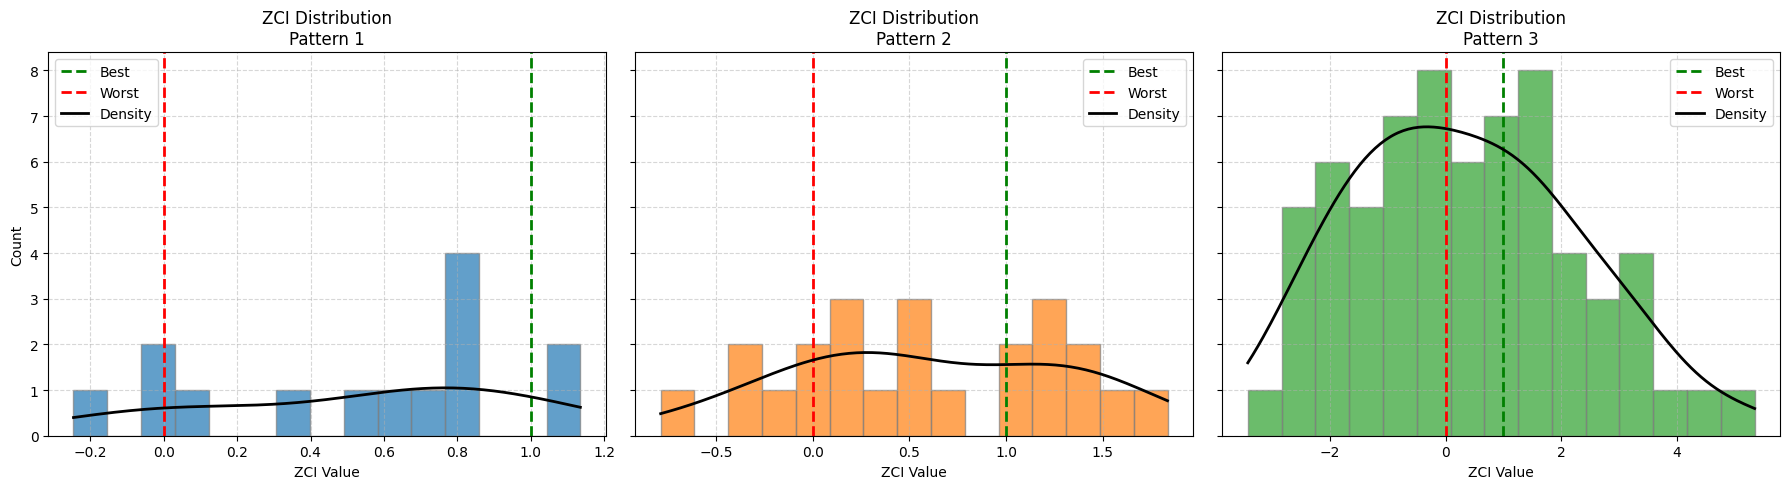
\includegraphics[width=\textwidth]{../results/preliminary_results/ZCI_distribution_across_clusters.png}
    \caption{ZCI Distribution across Clusters, showing the variation of ZCI scores within each cluster.}
    \label{fig:zci_distribution_across_clusters}
\end{figure}

The \textit{best} and \textit{worst} endpoints are used to perform Bray-Curtis ordination,
which scales the taxa compositions given the endpoints and compresses the 16 taxa variables into a single value
to reflect the distance to the endpoints.
In each cluster, the resulting ZCI scores of the two endpoints were converted to 0 and 1, 
and the ZCI scores of other sites were transformed with the same scale, which is not a [0 ,1] range mapping,
but a value-based ZCI score that reflects the distance to the endpoints.

Figure \textcolor{blue}{\ref{fig:zci_vs_stress_and_taxa_abundance}} 
shows the scatter plot of ZCI scores vs stress scores and the box plot of taxa abundance across taxa clusters.
One of the encouraging results is that the ZCI scores have correlation with the stress scores across three clusters,
and the scatter plots in Figure \textcolor{blue}{\ref{fig:zci_vs_stress_and_taxa_abundance}}
show very likely correlations between ZCI scores and stress scores.

And to the lower half of the Figure \textcolor{blue}{\ref{fig:zci_vs_stress_and_taxa_abundance}},
we hope to see the taxa abundance distribution differences across the three clusters 
due to the different environmental conditions. 
But this boxplot is not comparable to the boxplot shown in Figure \textcolor{blue}{\ref{fig:taxa_abundance_by_site_label}},
because the Figure \textcolor{blue}{\ref{fig:taxa_abundance_by_site_label}} is the taxa abundance distribution controlled by 
the human disturbance levels, while the Figure \textcolor{blue}{\ref{fig:zci_vs_stress_and_taxa_abundance}}
shows the taxa abundance distribution controlled by environmental conditions.
The differences in controlled conditions make it unreasonable to compare these two boxplots, even though
they may look similar.

\begin{figure}[!h]
    \centering
    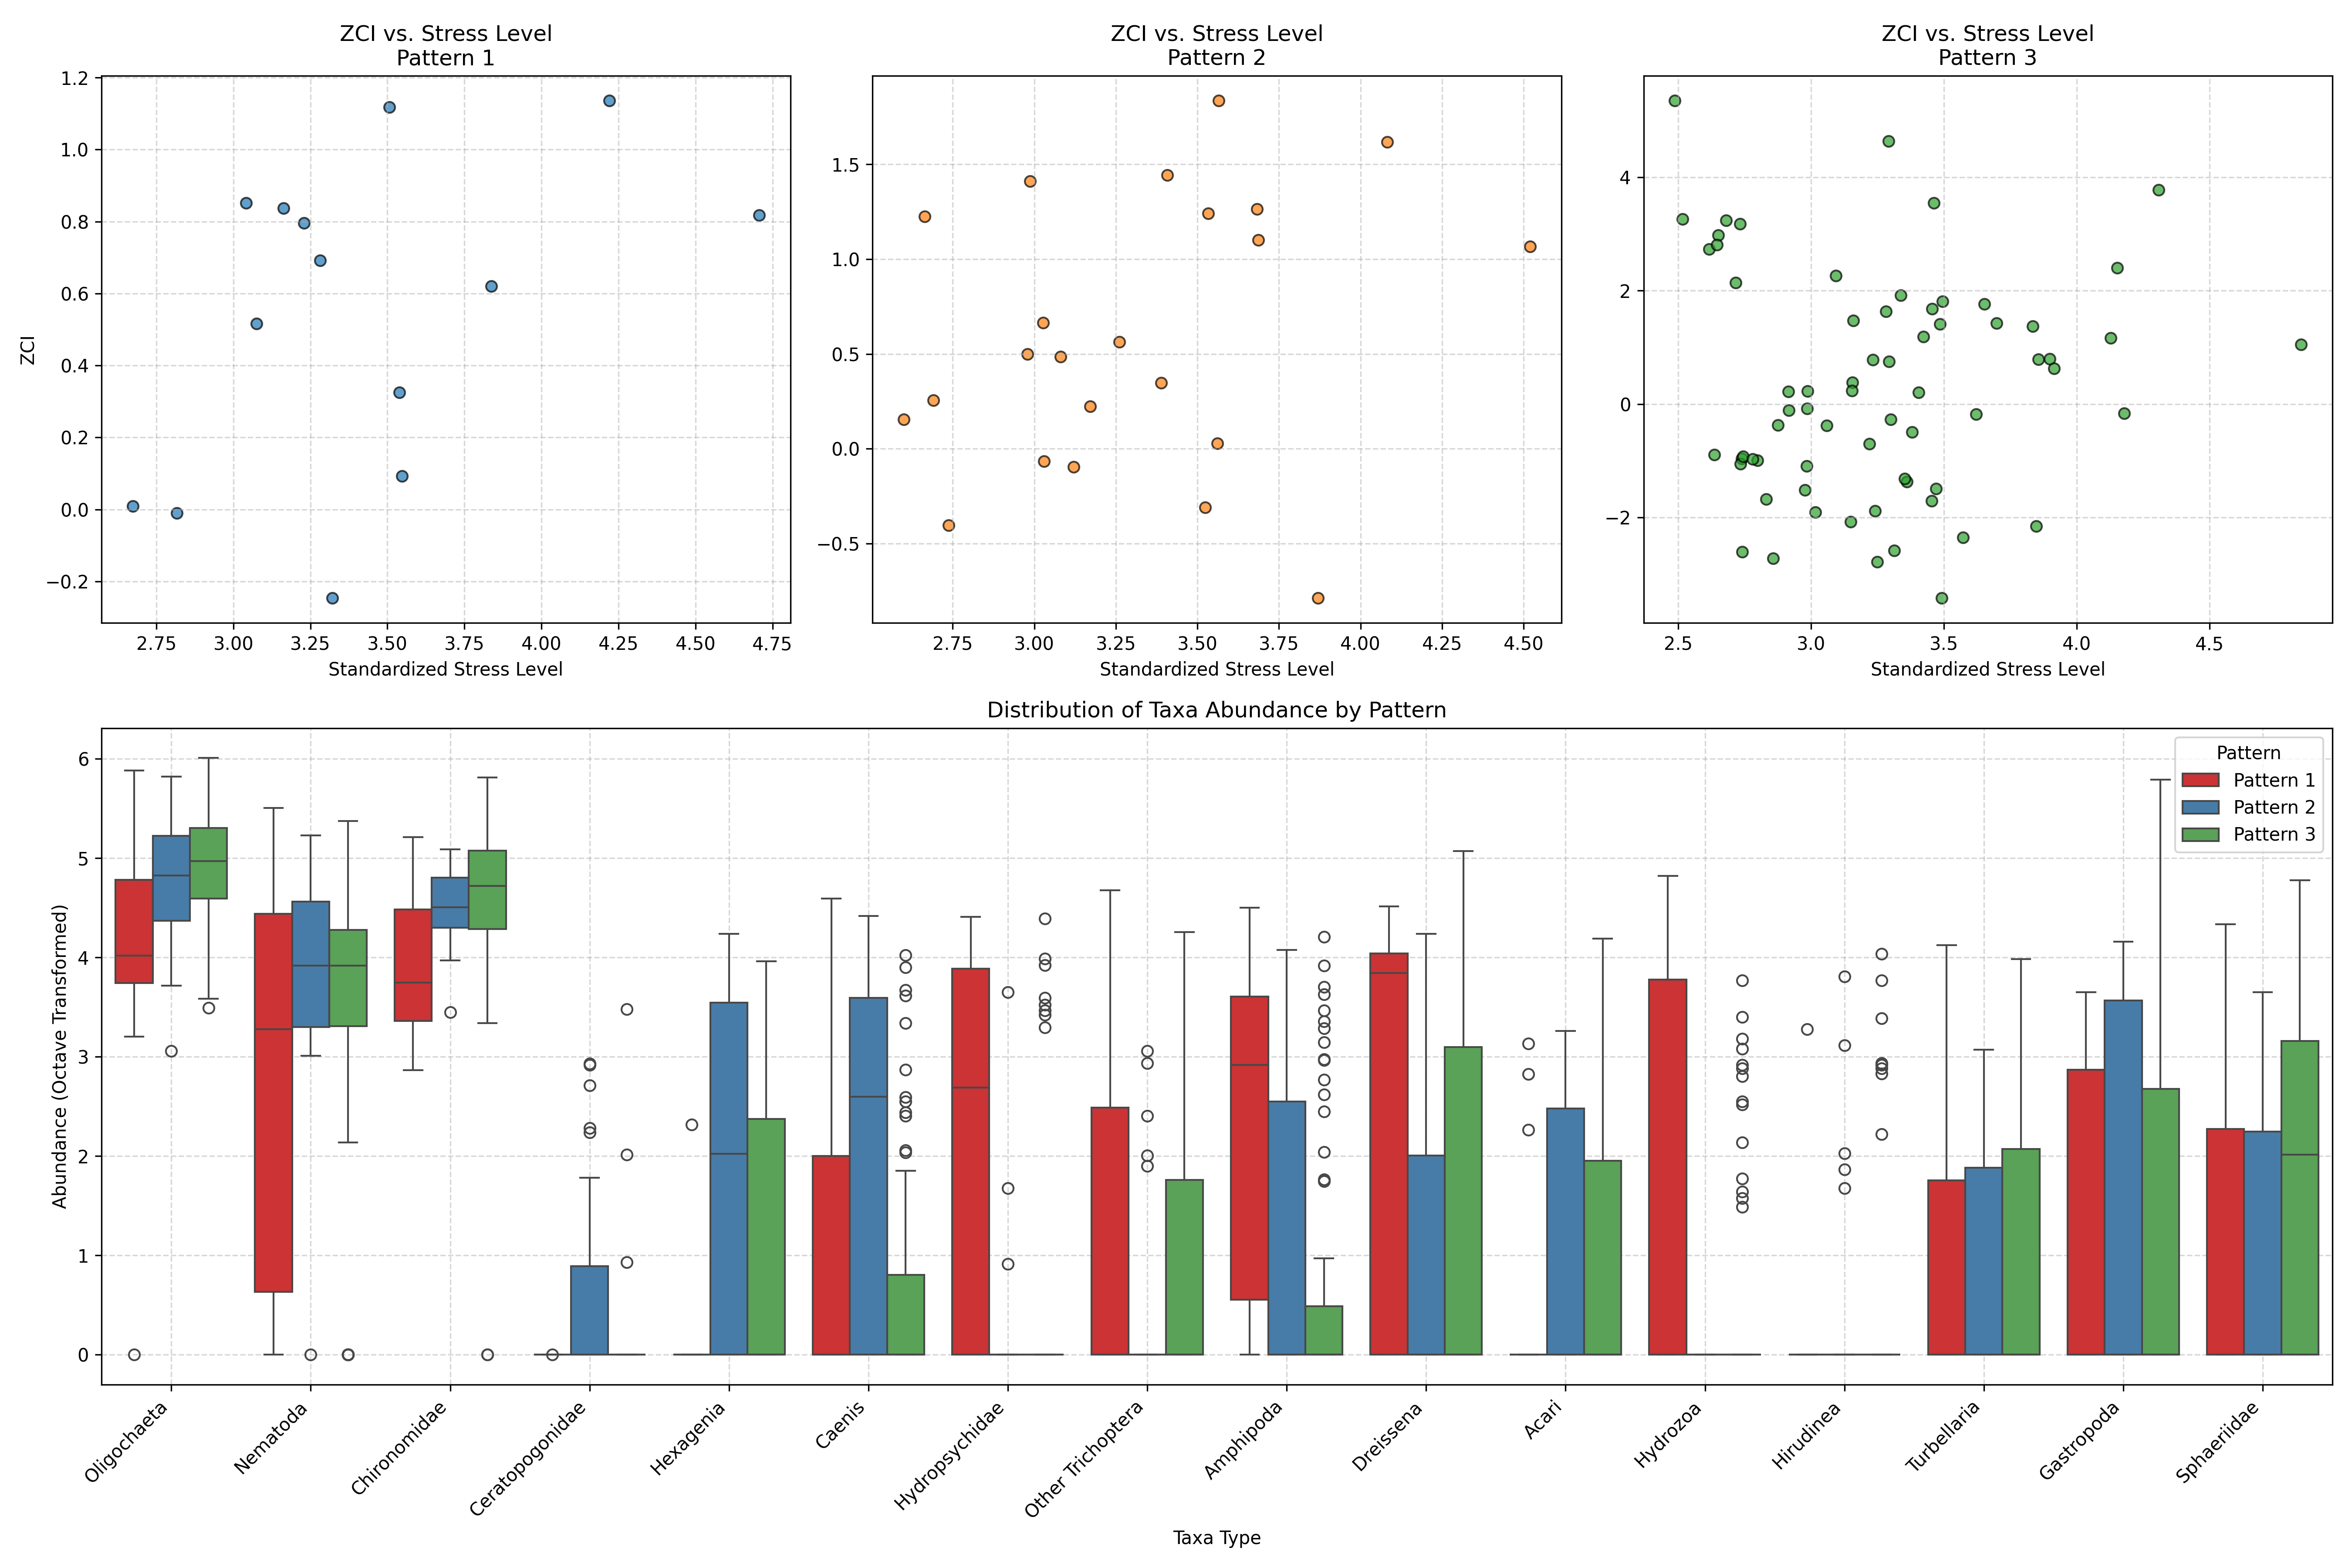
\includegraphics[width=\textwidth]{../results/preliminary_results/zci_vs_stress_and_taxa_abundance.png}
    \caption{ZCI vs Stress Scores and the Distribution of Taxa Abundance across Taxa Patterns}
    \label{fig:zci_vs_stress_and_taxa_abundance}
\end{figure}

\subsection{Evaluate the ZCI vs SumRel relationship by quantile regression}

Now, there were complete ZCI scores and stress scores for all sites,
and their relationships were evaluated by quantile regression across clusters.

To this step, within each cluster, I have had the ZCI scores and stress scores for each site,
and they are value-based scores so that simple linear or quantile regression can be applied to them.

A quantile regression was applied to the ZCI scores and stress scores within each cluster 
to evaluate the relationship between them, a bias-corrected bootstrapping method was applied 
to estimate the confidence intervals of the quantile regression coefficients.

Figure \textcolor{blue}{\ref{fig:qrm_quantile_regression_pattern_1}} to Figure \textcolor{blue}{\ref{fig:qrm_quantile_regression_pattern_3}}
show the quantile regression results of different \(\tau\) values for each cluster.
Stress score of 4, the horizontal red line, is marked as degraded threshold for all three clusters for convenience,
and there are one or two visible quantile regression lines crossing the threshold value.
The intersection of a \(\tau^*\) level quantile regression line and the horizontal red line
provides the estimated percent of samples conditioned on the corresponding ZCI score
to be less than or equal to the degraded threshold.

The one-side p-value for null hypothesis that the relative stress level
conditional on such ZCI score \(x_k^*\) is less than the degraded threshold \(H_0: \delta X < x_k^*\)
can be computed as \(1 - \tau^*\). 
As a potential example like Figure \textcolor{blue}{\ref{fig:qrm_quantile_regression_pattern_1}},
quantile regression lines of \(\tau = 1\) and \(\tau = 0.77\) cross the degraded threshold
at around \(ZCI = 0.25\) and \(ZCI = 0.8\) respectively, such results indicate that
there are other quantile regression lines intersecting the degraded threshold between
the ZCI scores of 0.25 and 0.8, and these quantile levels must fall between 0.77 and 1.

In Appendix, there are piecewise quantile regression results for each cluster and 
other techniques, like bootstrap or synthetic data generation, can be applied to
enhance our understanding toward this inference method on top of the collected original data.

\begin{figure}
\centering
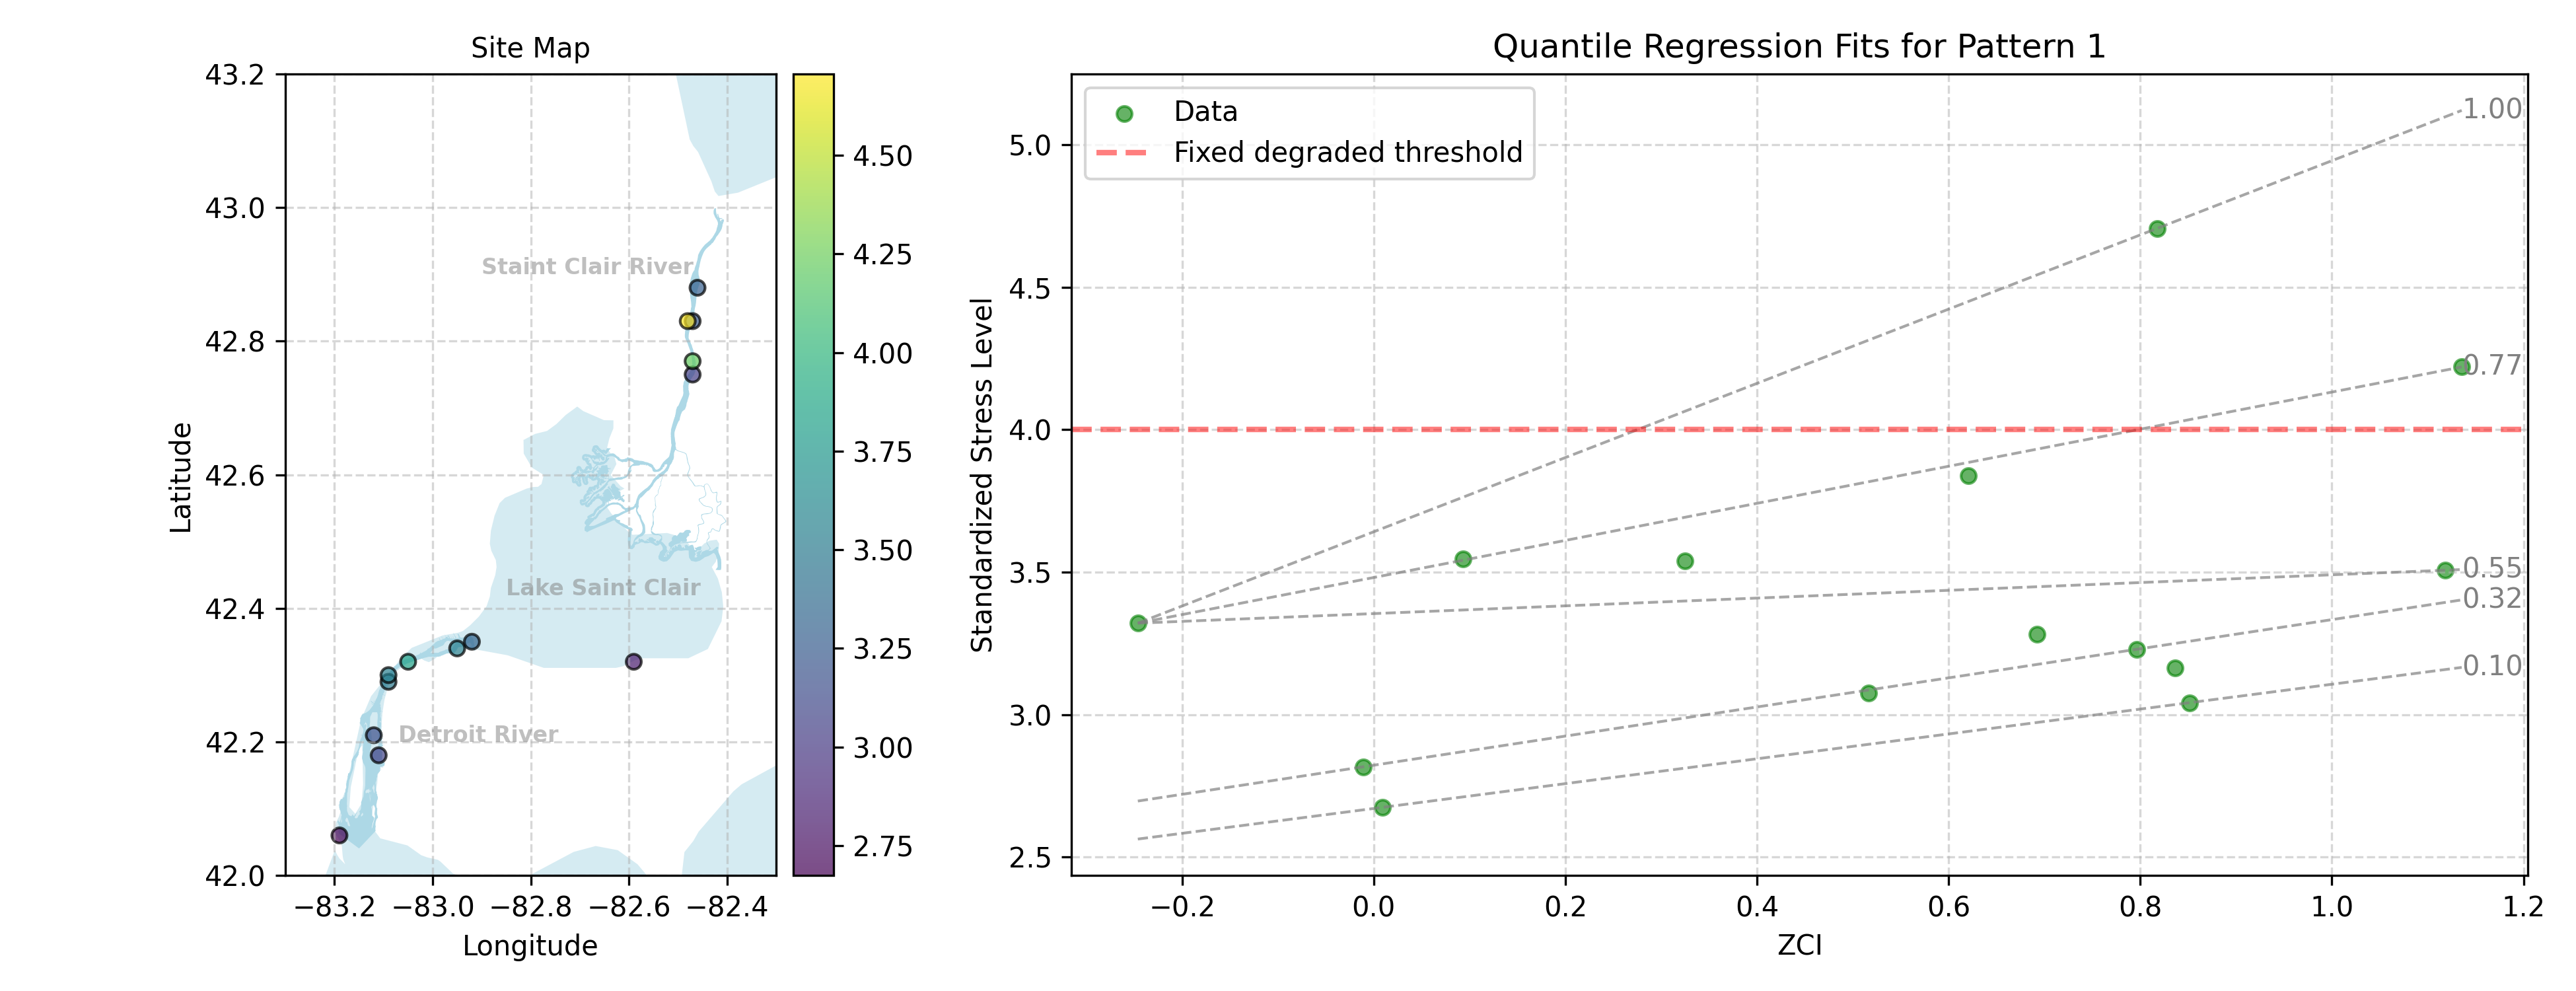
\includegraphics[width=\textwidth]{../results/preliminary_results/qrm_quantile_regression_pattern_1.png}
\caption{Quantile Regression Results for Cluster 1, showing the relationship between ZCI and stress scores.}
\label{fig:qrm_quantile_regression_pattern_1}
\end{figure}

\begin{figure}
\centering
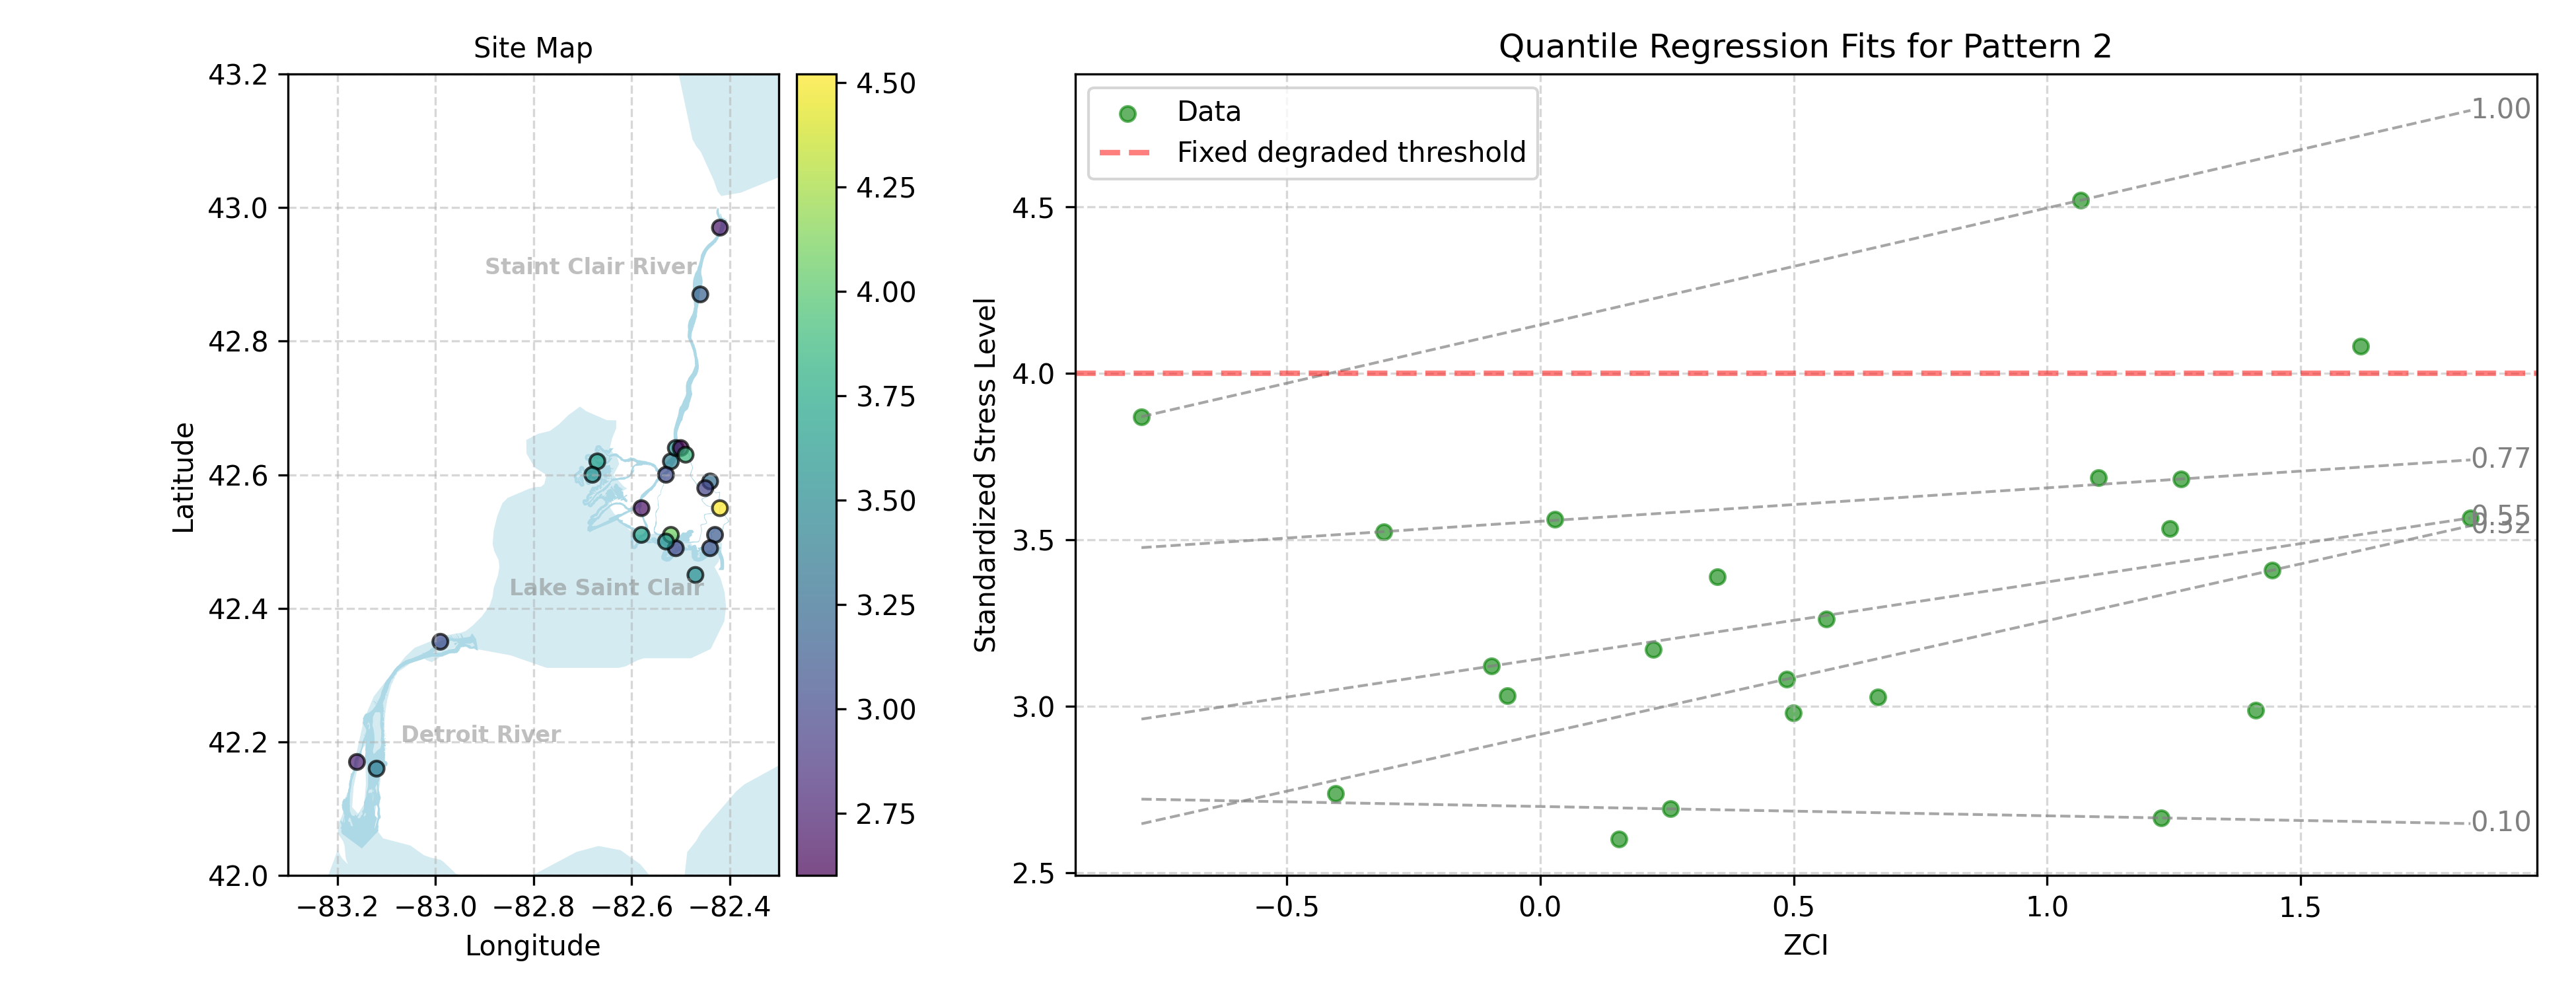
\includegraphics[width=\textwidth]{../results/preliminary_results/qrm_quantile_regression_pattern_2.png}
\caption{Quantile Regression Results for Cluster 2, showing the relationship between ZCI and stress scores.}
\label{fig:qrm_quantile_regression_pattern_2}
\end{figure}

\begin{figure}
\centering
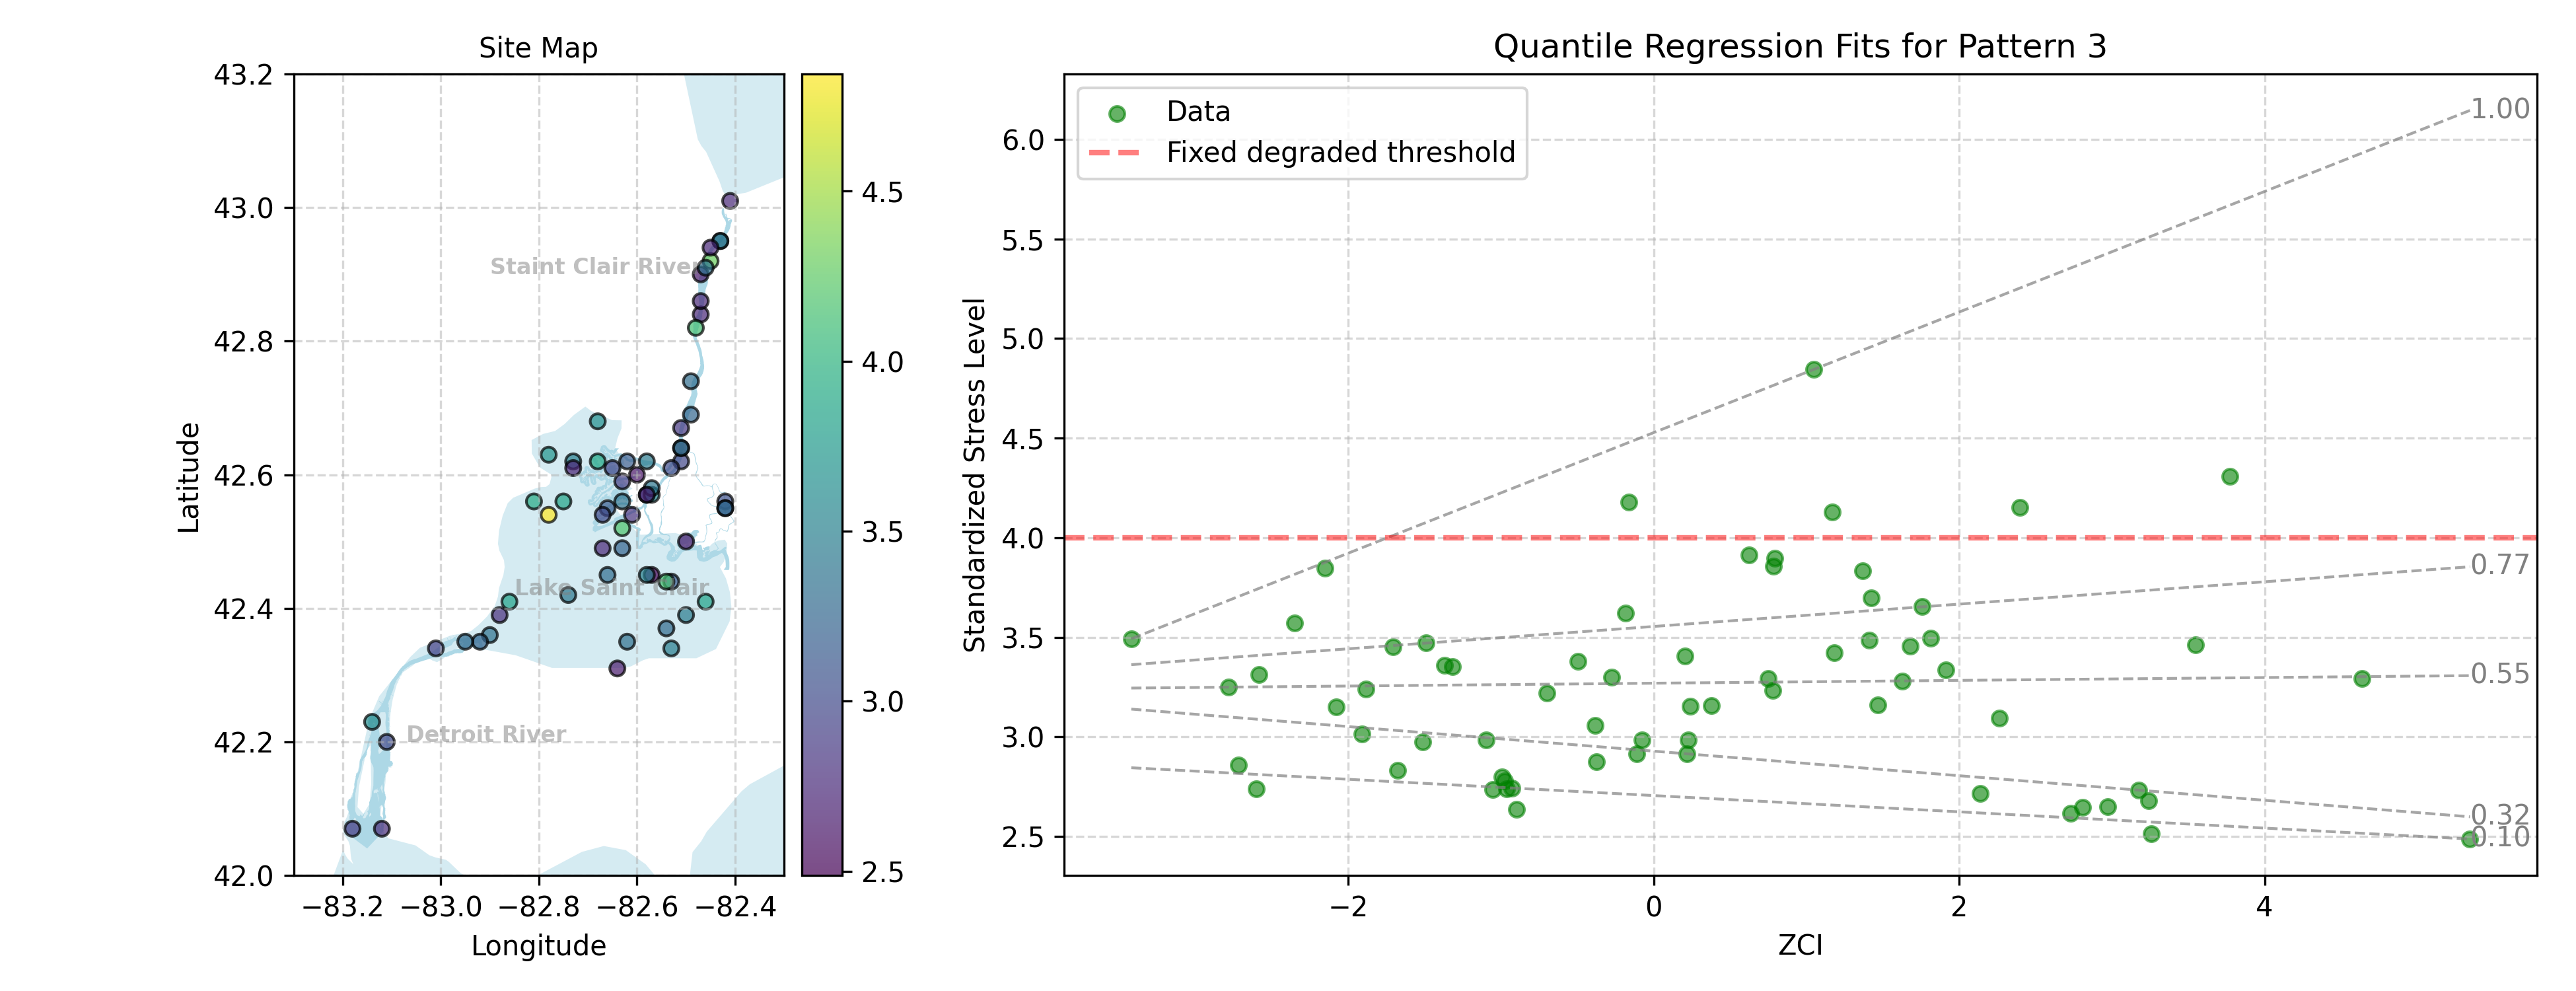
\includegraphics[width=\textwidth]{../results/preliminary_results/qrm_quantile_regression_pattern_3.png}
\caption{Quantile Regression Results for Cluster 3, showing the relationship between ZCI and stress scores.}
\label{fig:qrm_quantile_regression_pattern_3}
\end{figure}

\clearpage
\subsection{Extract spatial eigenvector by PCNM on simulated data}

PCNM (Principal Coordinates of Neighbour Matrices) provides a set of orthogonal spatial eigenvectors that can be used as 
covariates to model spatial structure (broad to fine scale) in subsequent analyses (e.g., quantile or generalized regression 
on taxa or stress scores). 
The workflow applied in the simulated data mirrors what will be done with true geographic information
(projected site coordinates of the Huron-Erie Corridor and Detroit River sites):

\begin{enumerate}
    \item Compute pairwise Euclidean (or great-circle then projected) distances among sites. Real coordinates will first be projected to an equal-area / appropriate planar CRS to avoid distortion.
    \item Determine a truncation threshold (here: maximum edge length of the minimum spanning tree / maximum nearest-neighbour distance) to ensure the distance graph is fully connected while suppressing unrealistically long links.
    \item Replace distances greater than the threshold with a large value (or leave as is in a truncated matrix) and convert to a truncated distance matrix.
    \item Apply double-centering (Gower centering) to obtain a spatially informed matrix whose eigen decomposition yields orthogonal axes ordered from broad (large-scale) to fine (small-scale) spatial structures.
    \item Retain eigenvectors with positive spatial autocorrelation (screened by Moran's I \(> 0\) and, if needed, significance tests under permutation).
    These become the candidate spatial predictors (denoted S). A subset S$_{sel}$ is chosen to avoid overfitting (e.g., forward selection with adjusted R$^2$ or information criteria) when added to ecological models.
\end{enumerate}

The three simulation figures illustrate how sampling design influences the scale and appearance of retained eigenvectors:

\textbf{Figure \textcolor{blue}{\ref{fig:pcnm_simulation_1d_equally_spaced}}} (1D regular): With evenly spaced sites along a line, early (broad) eigenvectors resemble low-frequency sine/cosine waves capturing gradual longitudinal gradients. Progressively higher-order (not all shown) eigenvectors would introduce finer oscillations.
 The regular spacing produces a clean hierarchy of spatial scales.

\textbf{Figure \textcolor{blue}{\ref{fig:pcnm_simulation_2d_equally_spaced}}} (2D regular grid):
On a lattice, broad-scale eigenvectors express smooth surfaces across both axes. 
Subsequent eigenvectors increasingly capture checkerboard or banded patterns that 
partition the grid into larger then smaller spatial patches. 
The symmetry of the grid yields balanced representation of directions,
which helps interpret broad-scale ecological gradients (e.g., upstream--downstream or depth-related trends) when transposed to real data.

\textbf{Figure \textcolor{blue}{\ref{fig:pcnm_simulation_2d_randomly_spaced}}} (2D irregular): 
Irregular (clustered / uneven) sampling causes eigenvectors to localize structure around denser site clusters and to stretch patterns across sparser regions. Broad-scale eigenvectors still reflect overall spatial extent, but intermediate components may appear asymmetric or warped because inter-site distances are uneven. This underscores the need, in the real dataset, to evaluate whether spatial coverage is sufficiently even; otherwise, model selection may prioritize localized eigenvectors that compensate for sampling gaps rather than true ecological gradients.

\textit{Application to real data}: 
Once applied to actual site coordinates, we will generate candidate PCNM eigenvectors, 
screen for positive spatial autocorrelation, and incorporate a subset into quantile
regression models. This aims to reduce spatial autocorrelation in residuals and
improve inference on non-spatial covariates while enabling spatially explicit 
variance interpretation.

The simulations therefore validate that the procedure recovers interpretable multi-scale patterns under contrasting sampling schemes and highlight considerations (threshold choice, uneven spacing) prior to deploying PCNM on the empirical dataset.

\begin{figure}[!h]
\centering
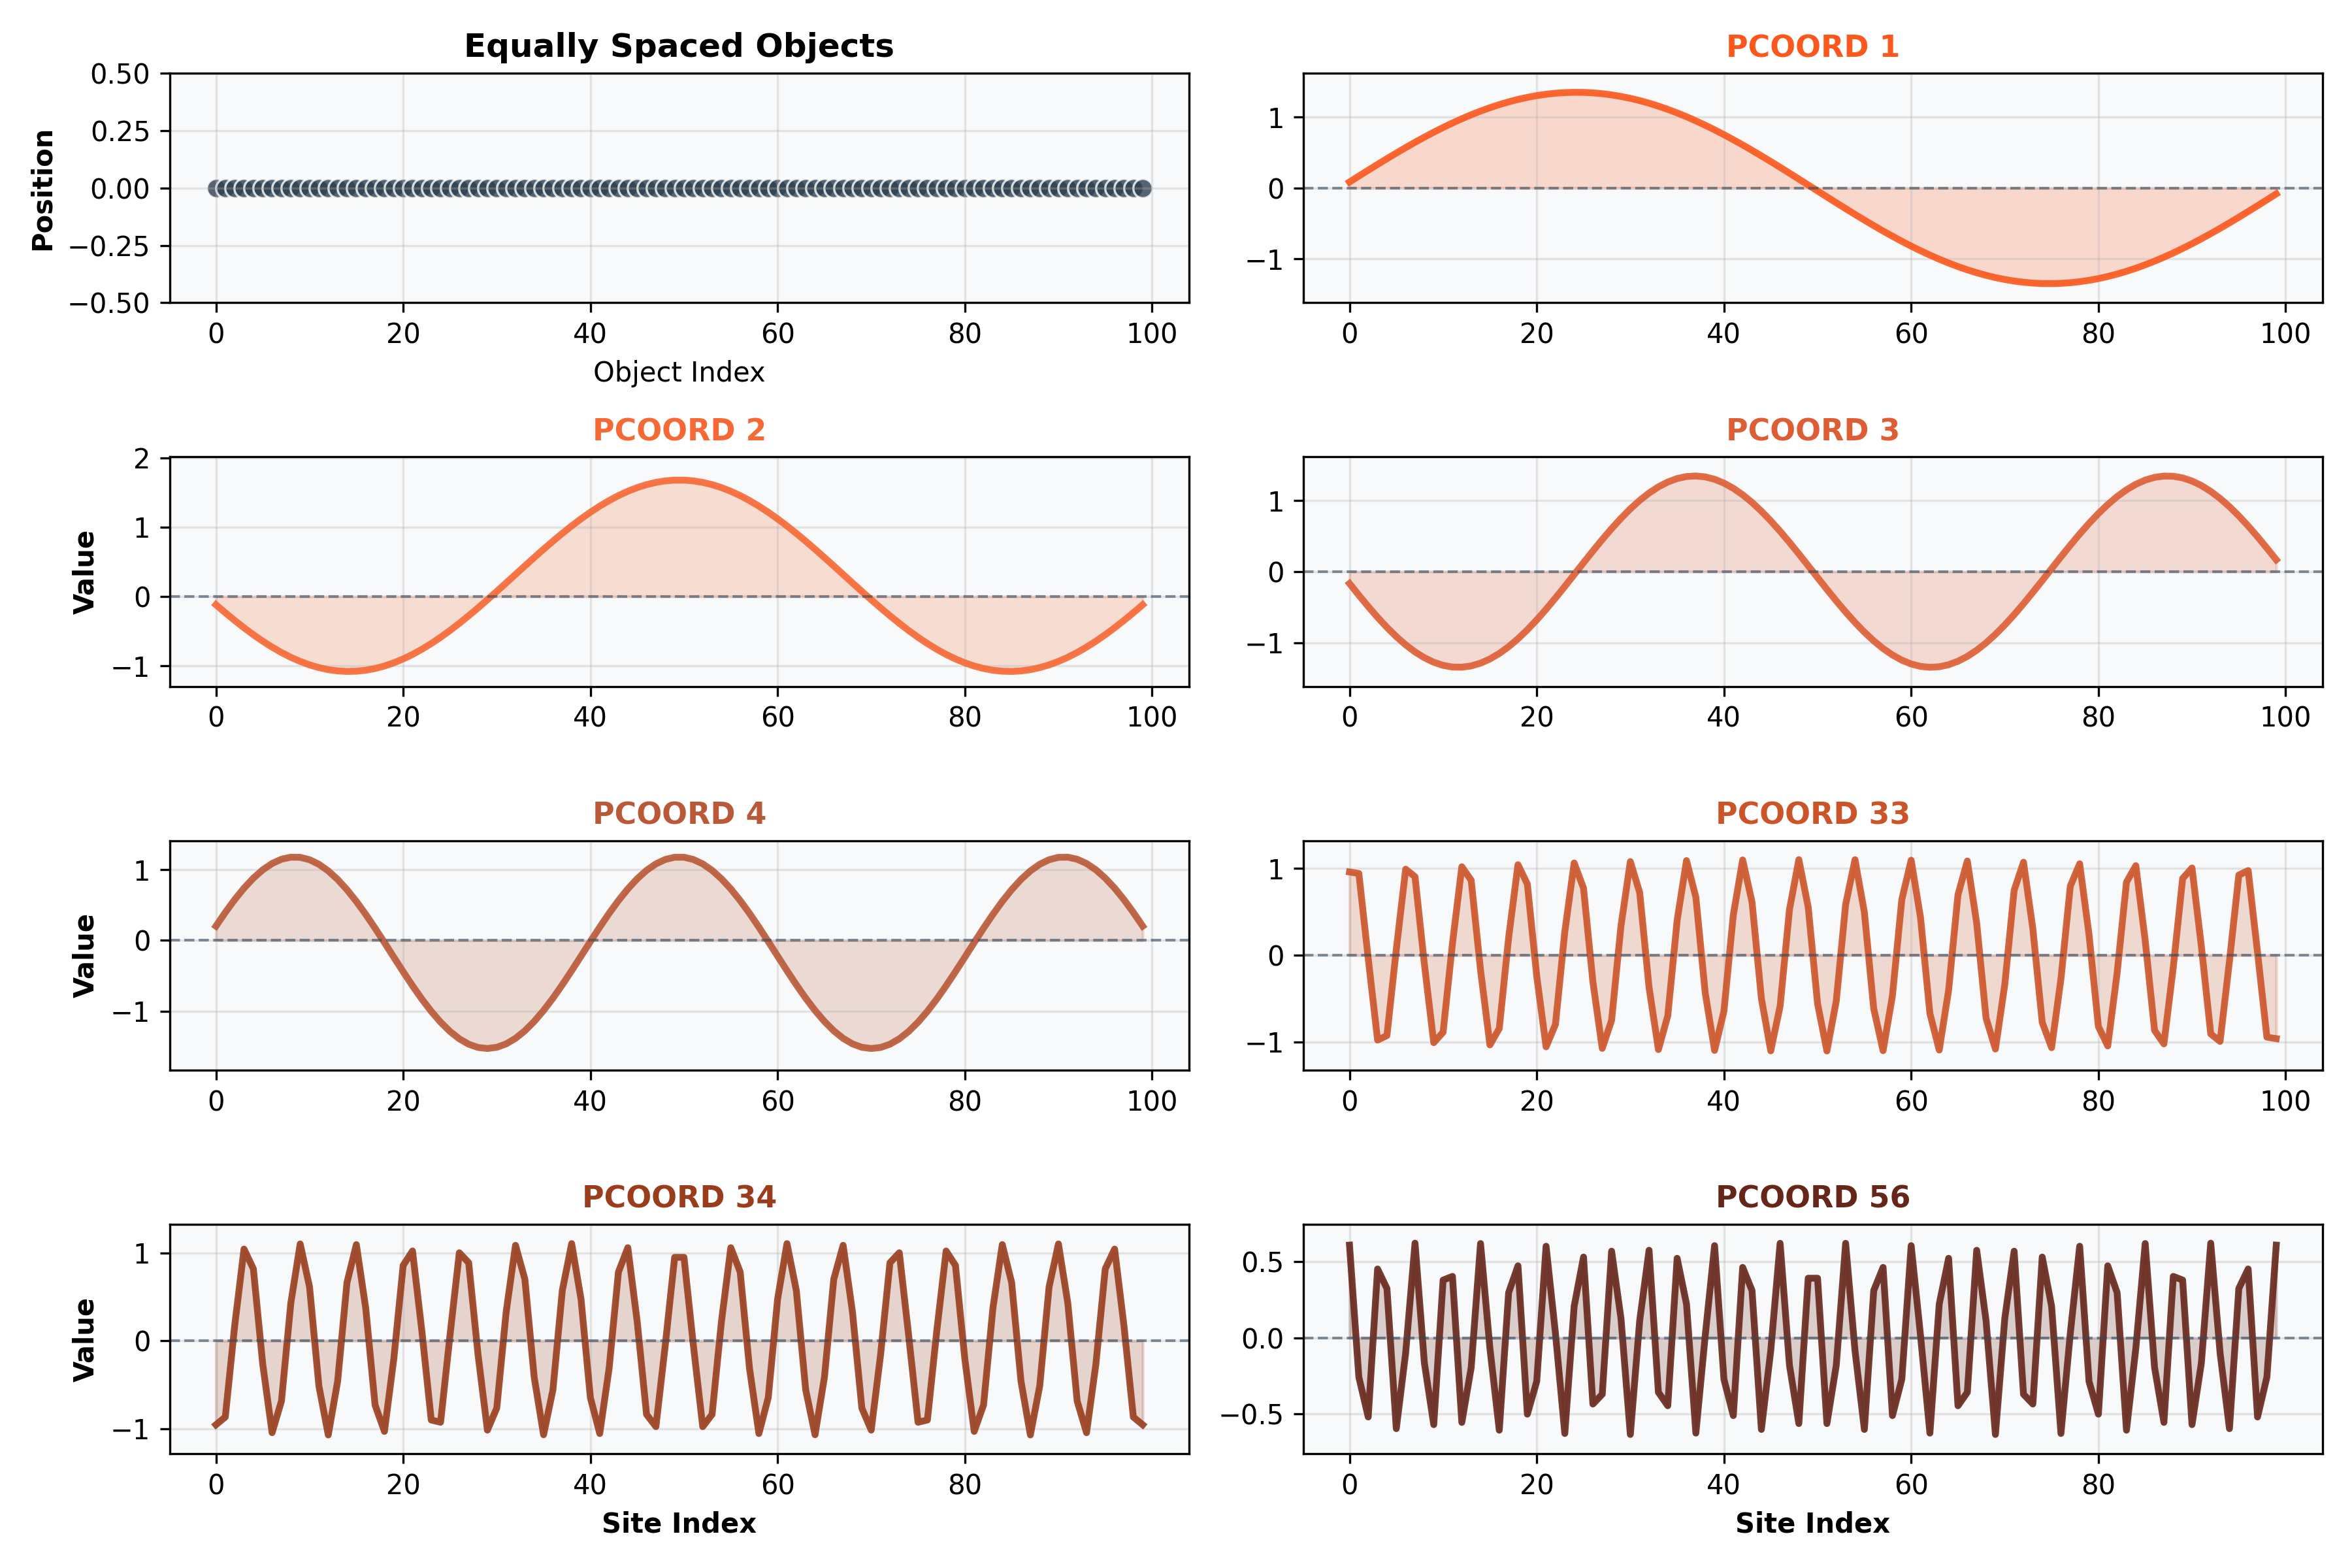
\includegraphics[width=0.9\textwidth]{../results/preliminary_results/pcnm_simulation_1d_equally_spaced.png}
\caption{PCNM simulation results for regular sampling in 1D space, showing the original sites and selected spatial eigenvectors.}
\label{fig:pcnm_simulation_1d_equally_spaced}
\end{figure}

\begin{figure}
\centering
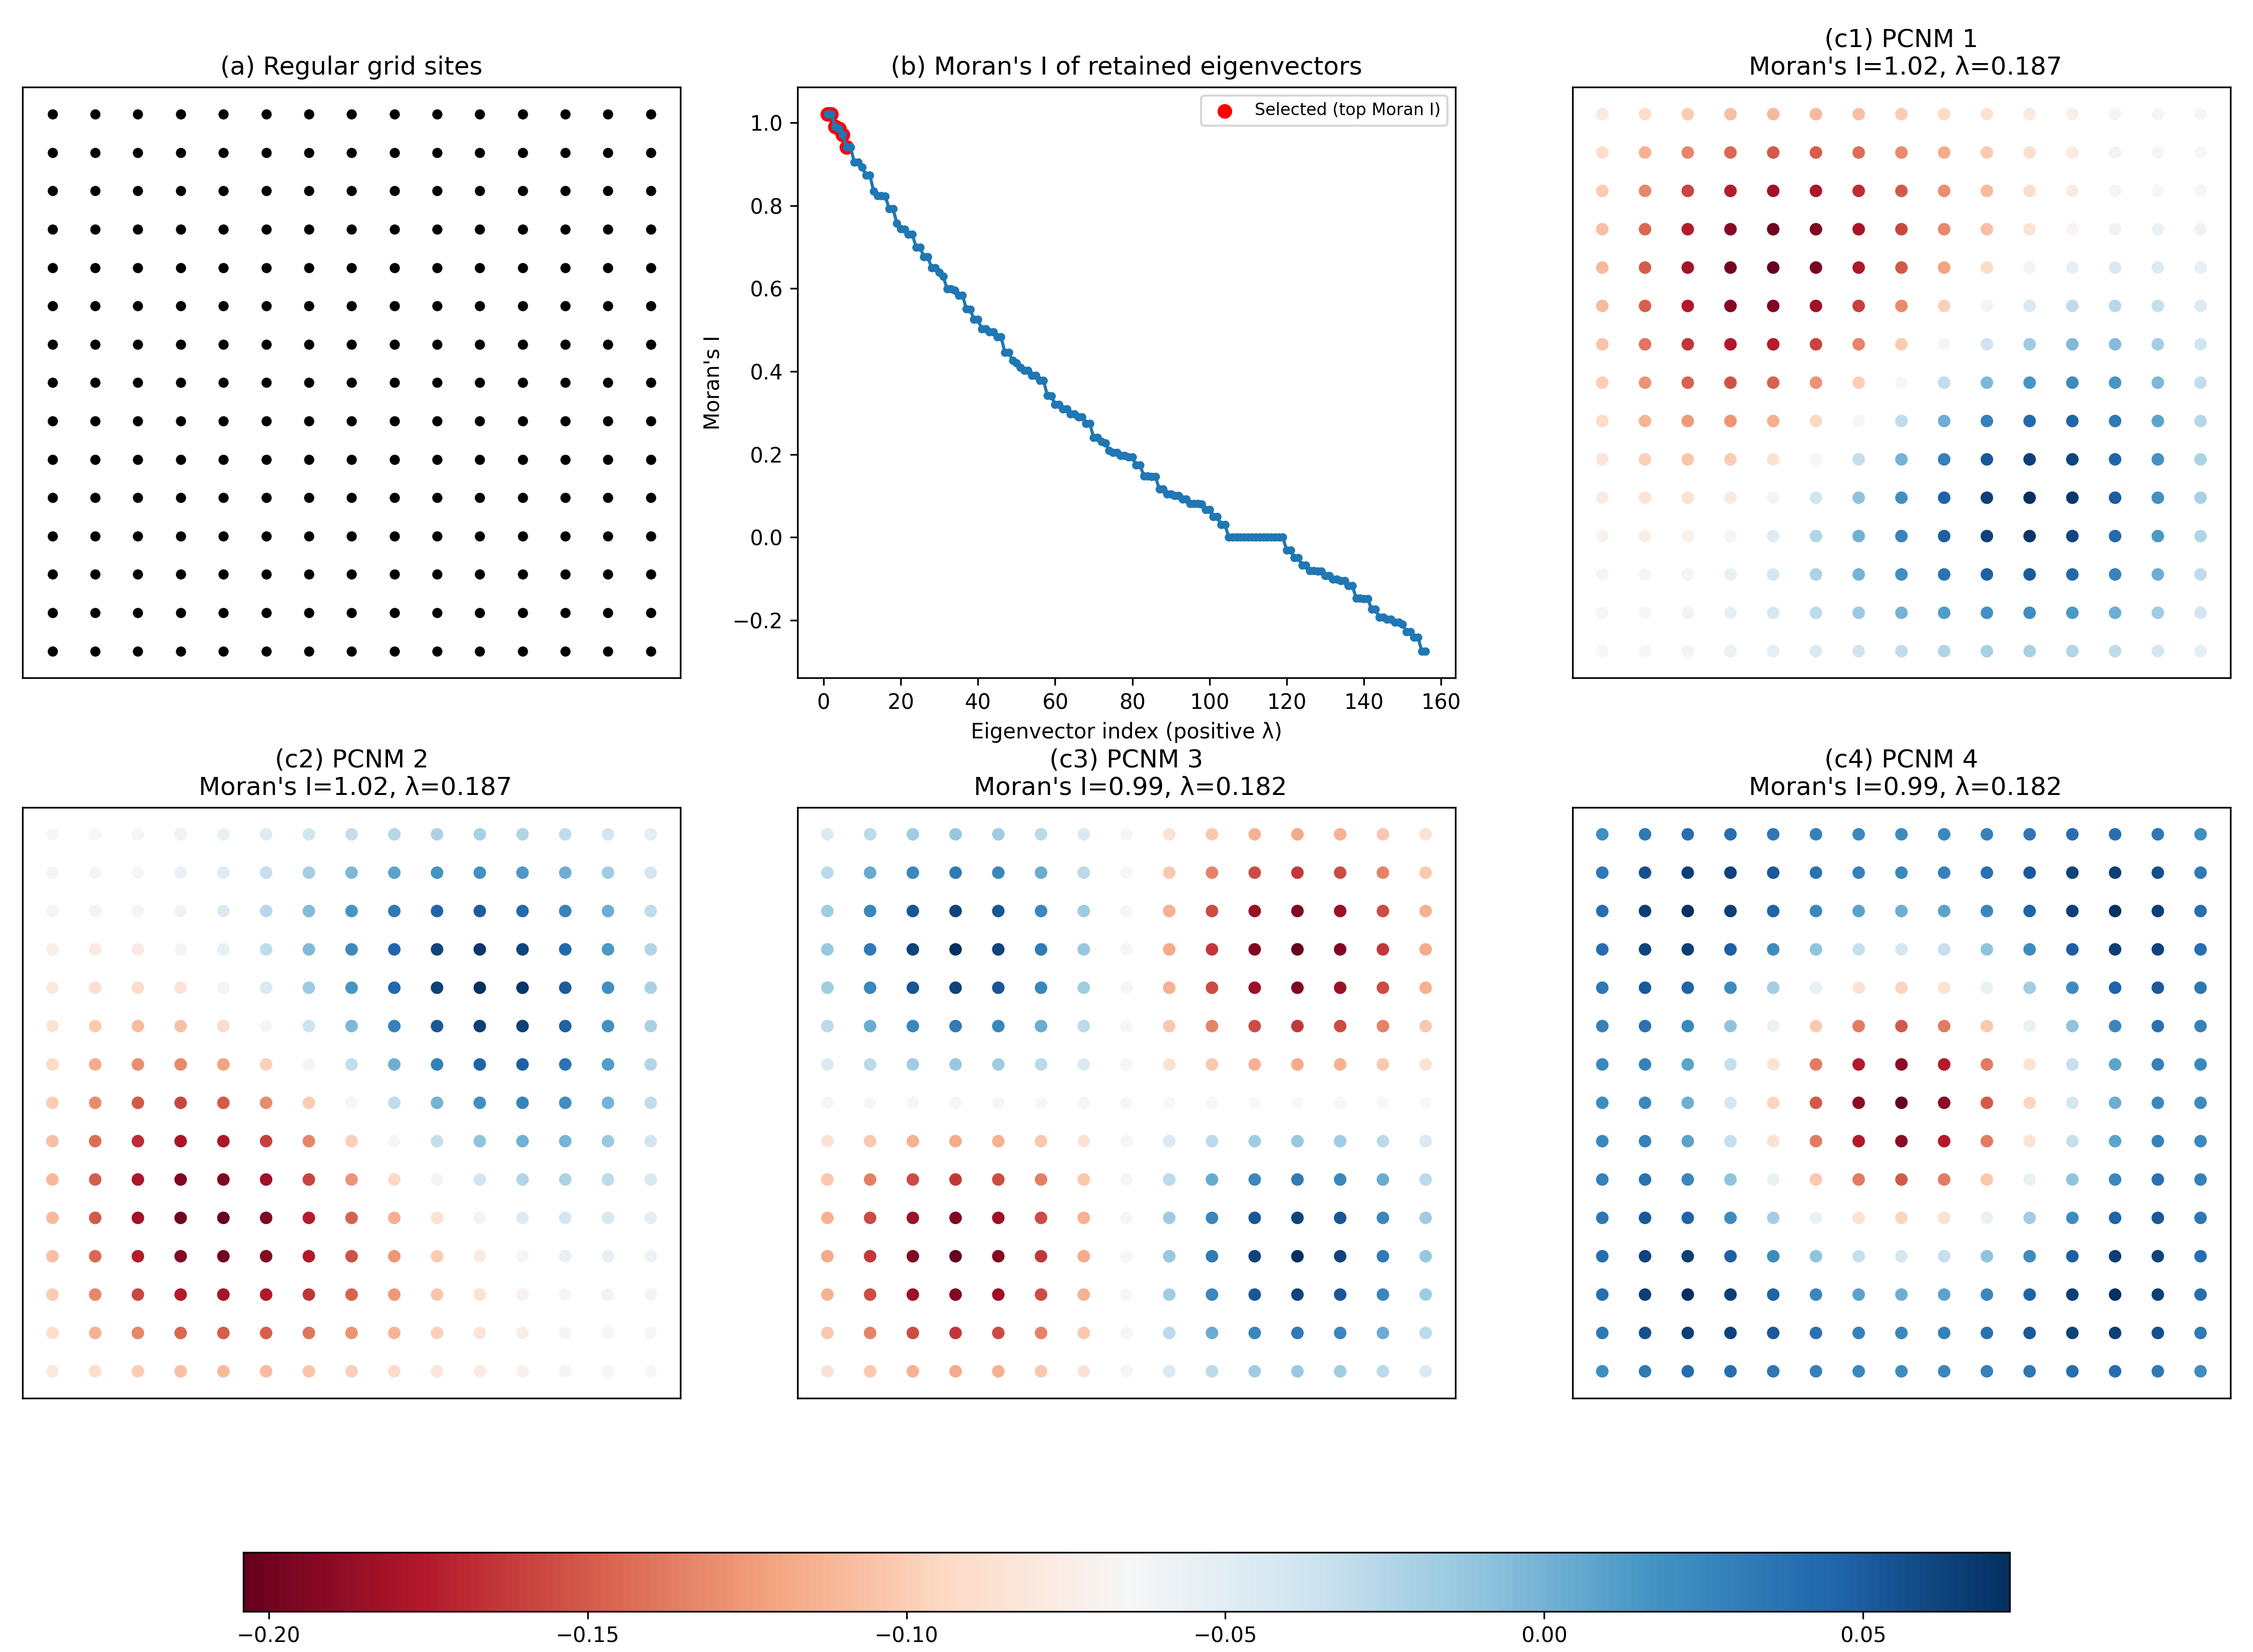
\includegraphics[width=0.9\textwidth]{../results/preliminary_results/pcnm_simulation_2d_equally_spaced.png}
\caption{PCNM simulation results for regular sampling in 2D space, showing the original sites and selected spatial eigenvectors.}
\label{fig:pcnm_simulation_2d_equally_spaced}
\end{figure}

\begin{figure}[!h]
\centering
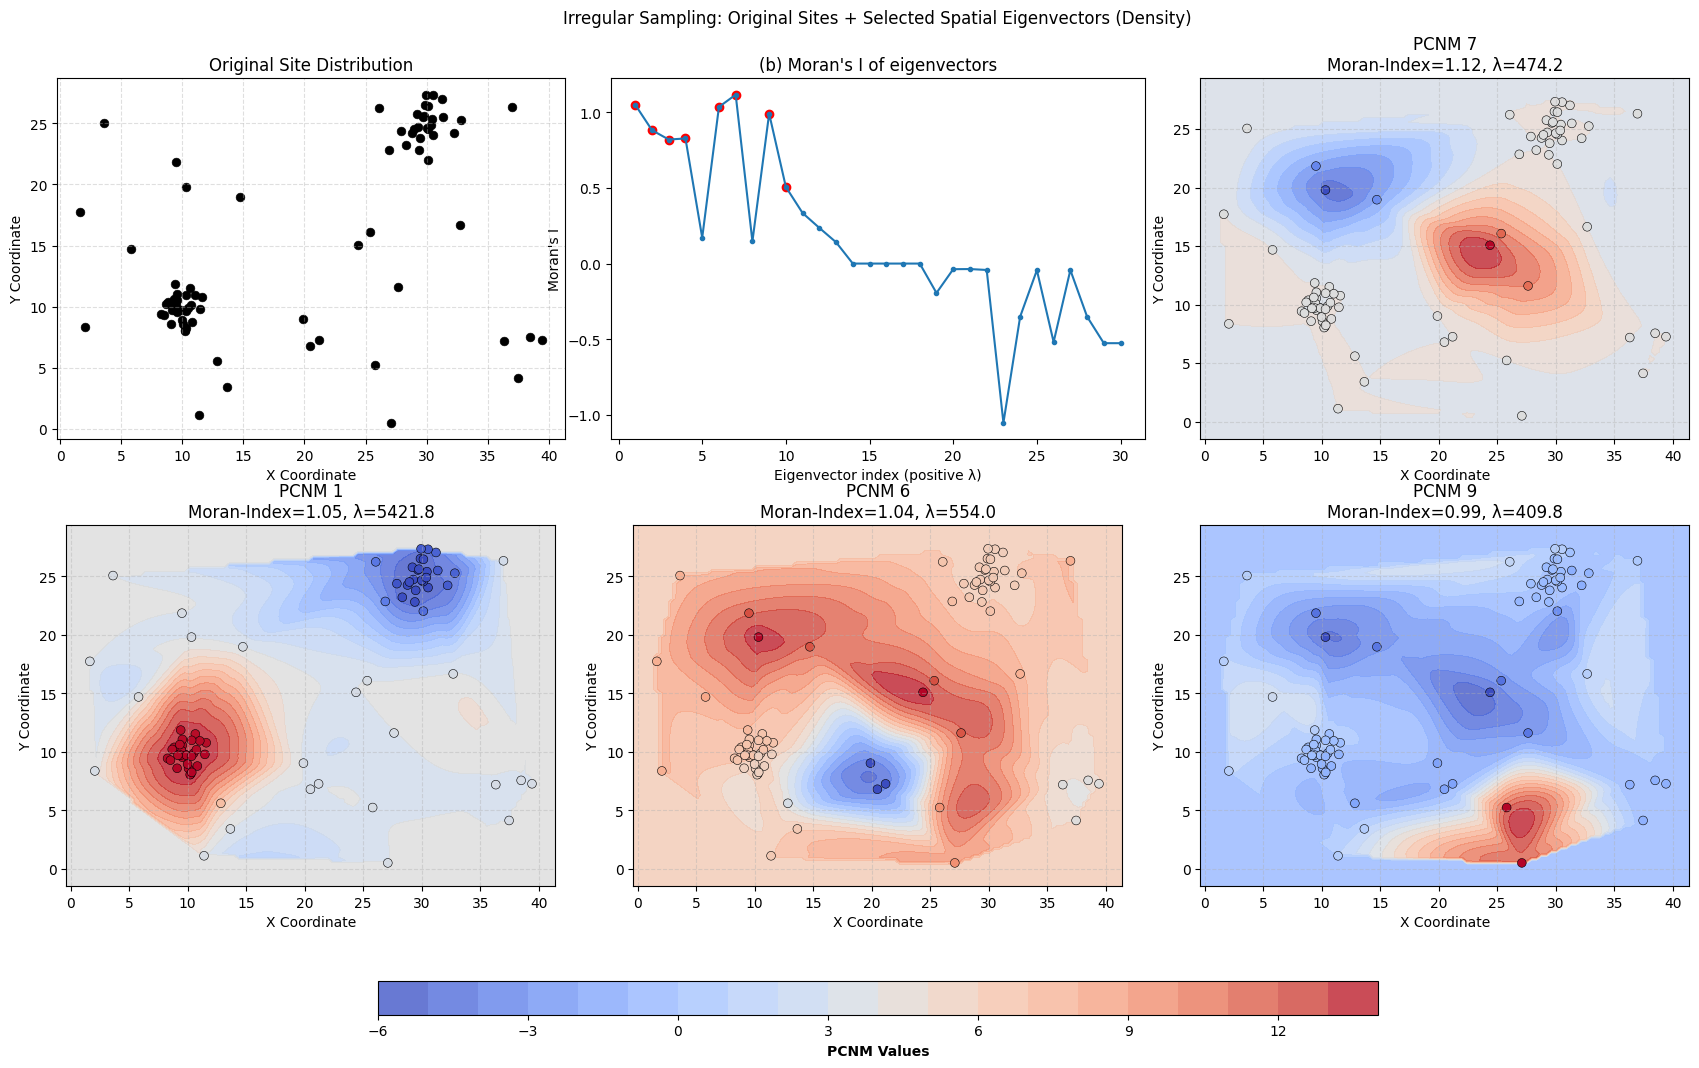
\includegraphics[width=0.9\textwidth]{../results/preliminary_results/pcnm_simulation_2d_randomly_spaced.png}
\caption{PCNM simulation results for irregular sampling in 2D space, showing the original sites and selected spatial eigenvectors.}
\label{fig:pcnm_simulation_2d_randomly_spaced}
\end{figure}

\begin{figure}[!h]
\centering
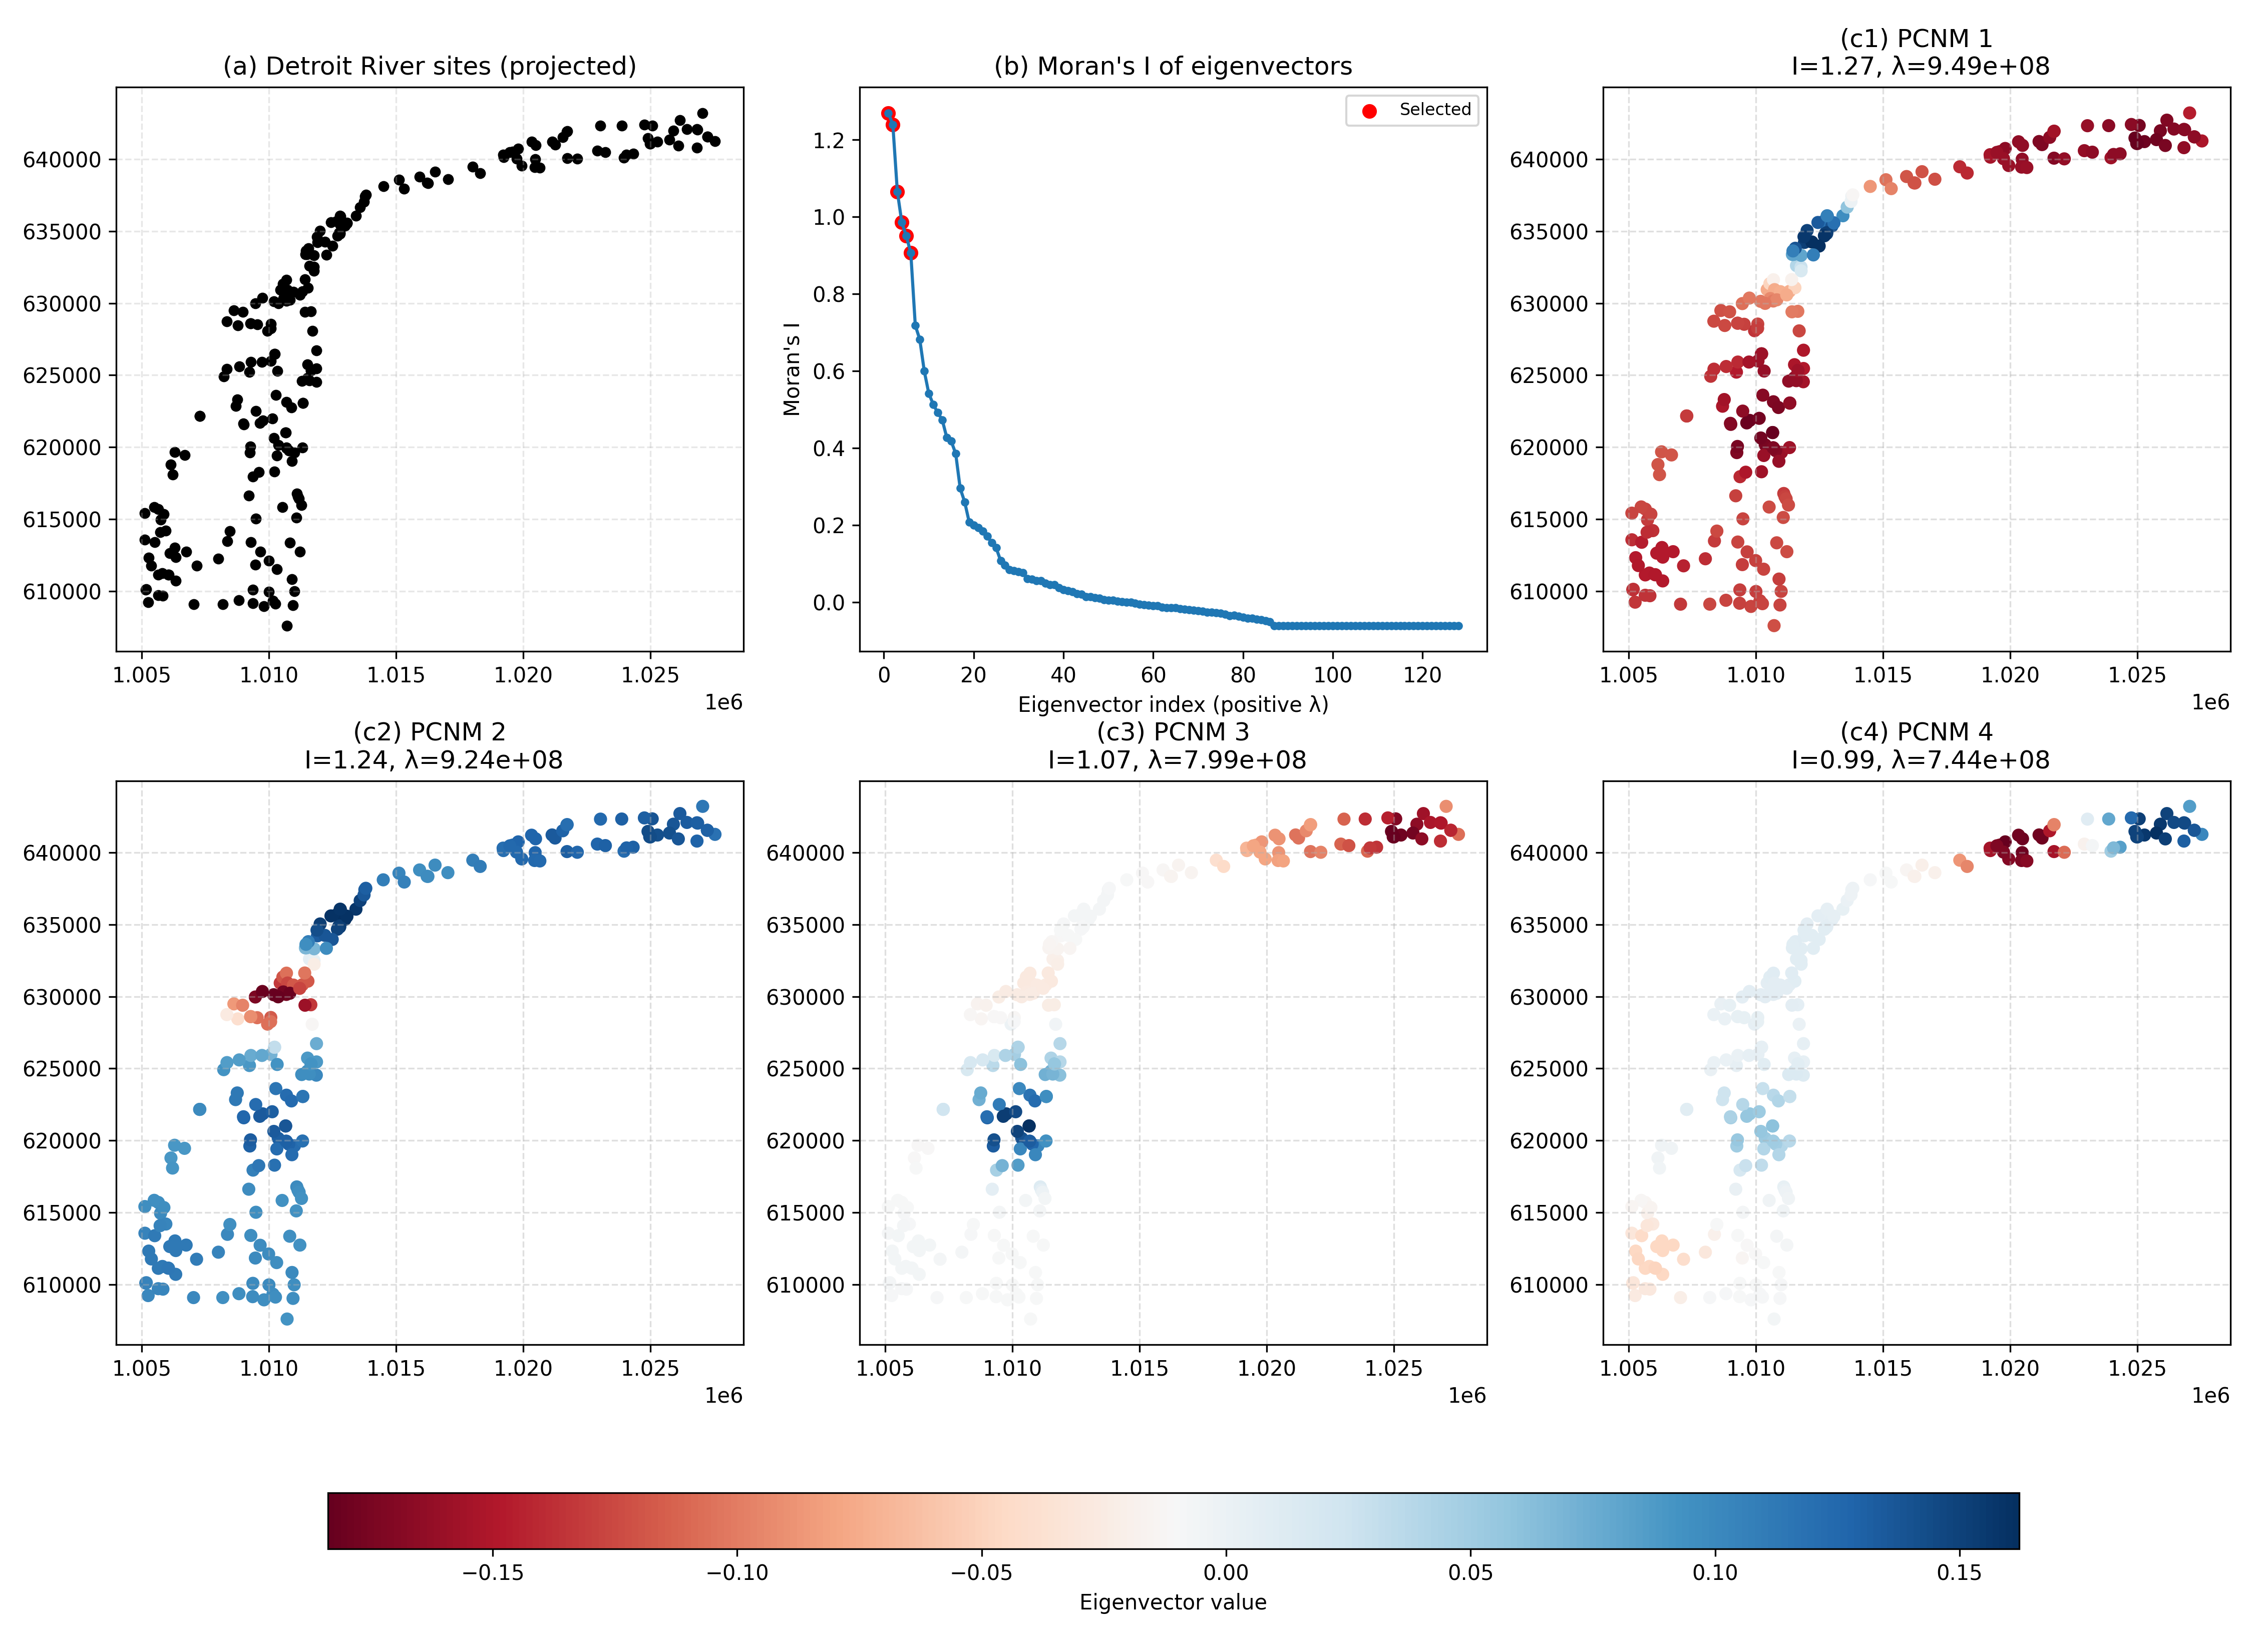
\includegraphics[width=0.9\textwidth]{../results/preliminary_results/pcnm_simulation_detroit_river.png}
\caption{PCNM simulation results for Detroit River site coordinates, showing the original sites and selected spatial eigenvectors.}
\label{fig:pcnm_simulation_detroit_river}
\end{figure}

\clearpage
\subsection{Power and sensitivity analysis on quantile regression with simulated data}

This simulation evaluates two practical design questions for a piecewise (hinge) quantile regression intended for later ecological inference: (i) how precisely can the slope ($\beta_1$) and post-break change ($\delta$) be recovered across quantile levels $\tau$, and (ii) what sample size is required to attain acceptable power ($\geq 0.8$) to detect a true hinge effect at a high conditional quantile while controlling the Type I error when the hinge effect is absent.

\textbf{Model and data generation.} We generated responses under a fixed breakpoint ($\kappa = 5$) hinge model
\[ Y = \beta_0 + \beta_1 X + \delta (X-\kappa)_+ + \varepsilon, \]
with parameters ($\beta_0=1.0$, $\beta_1=0.5$, $\delta=-0.6$) and heteroscedastic noise whose standard deviation increases linearly with $X$. A broad quantile grid $\tau \in \{0.05, 0.15, \ldots, 0.95\}$ allows inspection of effect heterogeneity across the conditional distribution.

\textbf{Estimation and hinge effect uncertainty.} For an initial sample ($n=500$) we fit separate quantile regressions (fixed $\kappa$) and constructed bootstrap confidence intervals ($B=300$) for the hinge coefficient $\delta_\tau$ using shared resampling indices across all $\tau$ within each bootstrap replicate. Sharing indices stabilizes cross-$\tau$ comparisons of $\delta_\tau$ and reduces Monte Carlo variability in the $\delta_\tau$ profile.

\textbf{Finite-population subsampling for precision.} To evaluate how precision scales with added observations we first generated a large synthetic ``population'' ($n=5000$) from the same model. Without replacement subsamples of sizes $n \in \{20, 50, 80, \ldots, 500\}$ were repeatedly drawn ($R=40$) and refit to obtain RMSE curves for the slope $\beta_{1\tau}$ and hinge $\delta_\tau$ relative to their generating values. This mimics augmenting an already characterized system rather than refitting to entirely new stochastic realizations, providing a conservative (finite-population) view of diminishing returns.

\textbf{Power and Type I operating characteristics.} For each candidate $n$, $L=70$ fresh datasets were simulated under (a) the alternative ($\delta = -0.6$) and (b) the null ($\delta = 0$). For every $\tau$ we computed a Wald statistic $|\hat{\delta}_\tau|/\text{SE}(\hat{\delta}_\tau)$ and declared detection if it exceeded $1.96$ (two-sided $\alpha \approx 0.05$). Bootstrap resampling of detection indicators ($B=350$) supplied $95\%$ confidence intervals for the empirical detection probability (power) and false positive rate (Type I). All proportions and interval bounds were clipped to $[0,1]$ for coherence. The high quantile $\tau=0.95$ was designated the primary design target because upper conditional responses often reflect limiting processes of ecological interest; the smallest $n$ achieving mean power $\geq 0.8$ at $\tau=0.95$ is reported as the recommended minimum sample size.

\textbf{Key results (Figure \textcolor{blue}{\ref{fig:power_sensitivity_analysis_simulation}} panels).}
(a) Fitted quantile functions (colored) closely envelop simulated data and track the deterministic mean (black), with clear post-break downward adjustment at higher $X$. (b) The $\delta_\tau$ profile shows moderately consistent negative hinge effects across mid-to-upper quantiles; bootstrap intervals exclude $0$ for higher $\tau$, indicating stronger evidence of a breakpoint effect in the upper tail. (c) RMSE declines rapidly up to roughly $n \approx 200$--$250$, after which gains flatten, suggesting diminishing precision returns beyond this range for $\tau=0.95$. (d) Power increases with $n$ and crosses $0.8$ at the recommended $n$ (vertical dashed line), while the empirical Type I error under $\delta=0$ remains near the nominal $0.05$ across sample sizes, confirming adequate test calibration under the simulation settings.

\textbf{Implications for study design.} These results provide a defensible sample size target and demonstrate that (i) synchronised bootstrap resampling enhances interpretability of cross-$\tau$ hinge effect patterns, (ii) finite-population style subsampling yields realistic diminishing returns guidance, and (iii) the proposed Wald-based detection maintains nominal error rates. Prior to applying the framework to empirical ZCI--stress analyses, sensitivity analyses around $\kappa$ mis-specification and noise structure can refine robustness expectations, but the current evidence supports proceeding with the indicated minimum $n$.

\begin{figure}[!h]
\centering
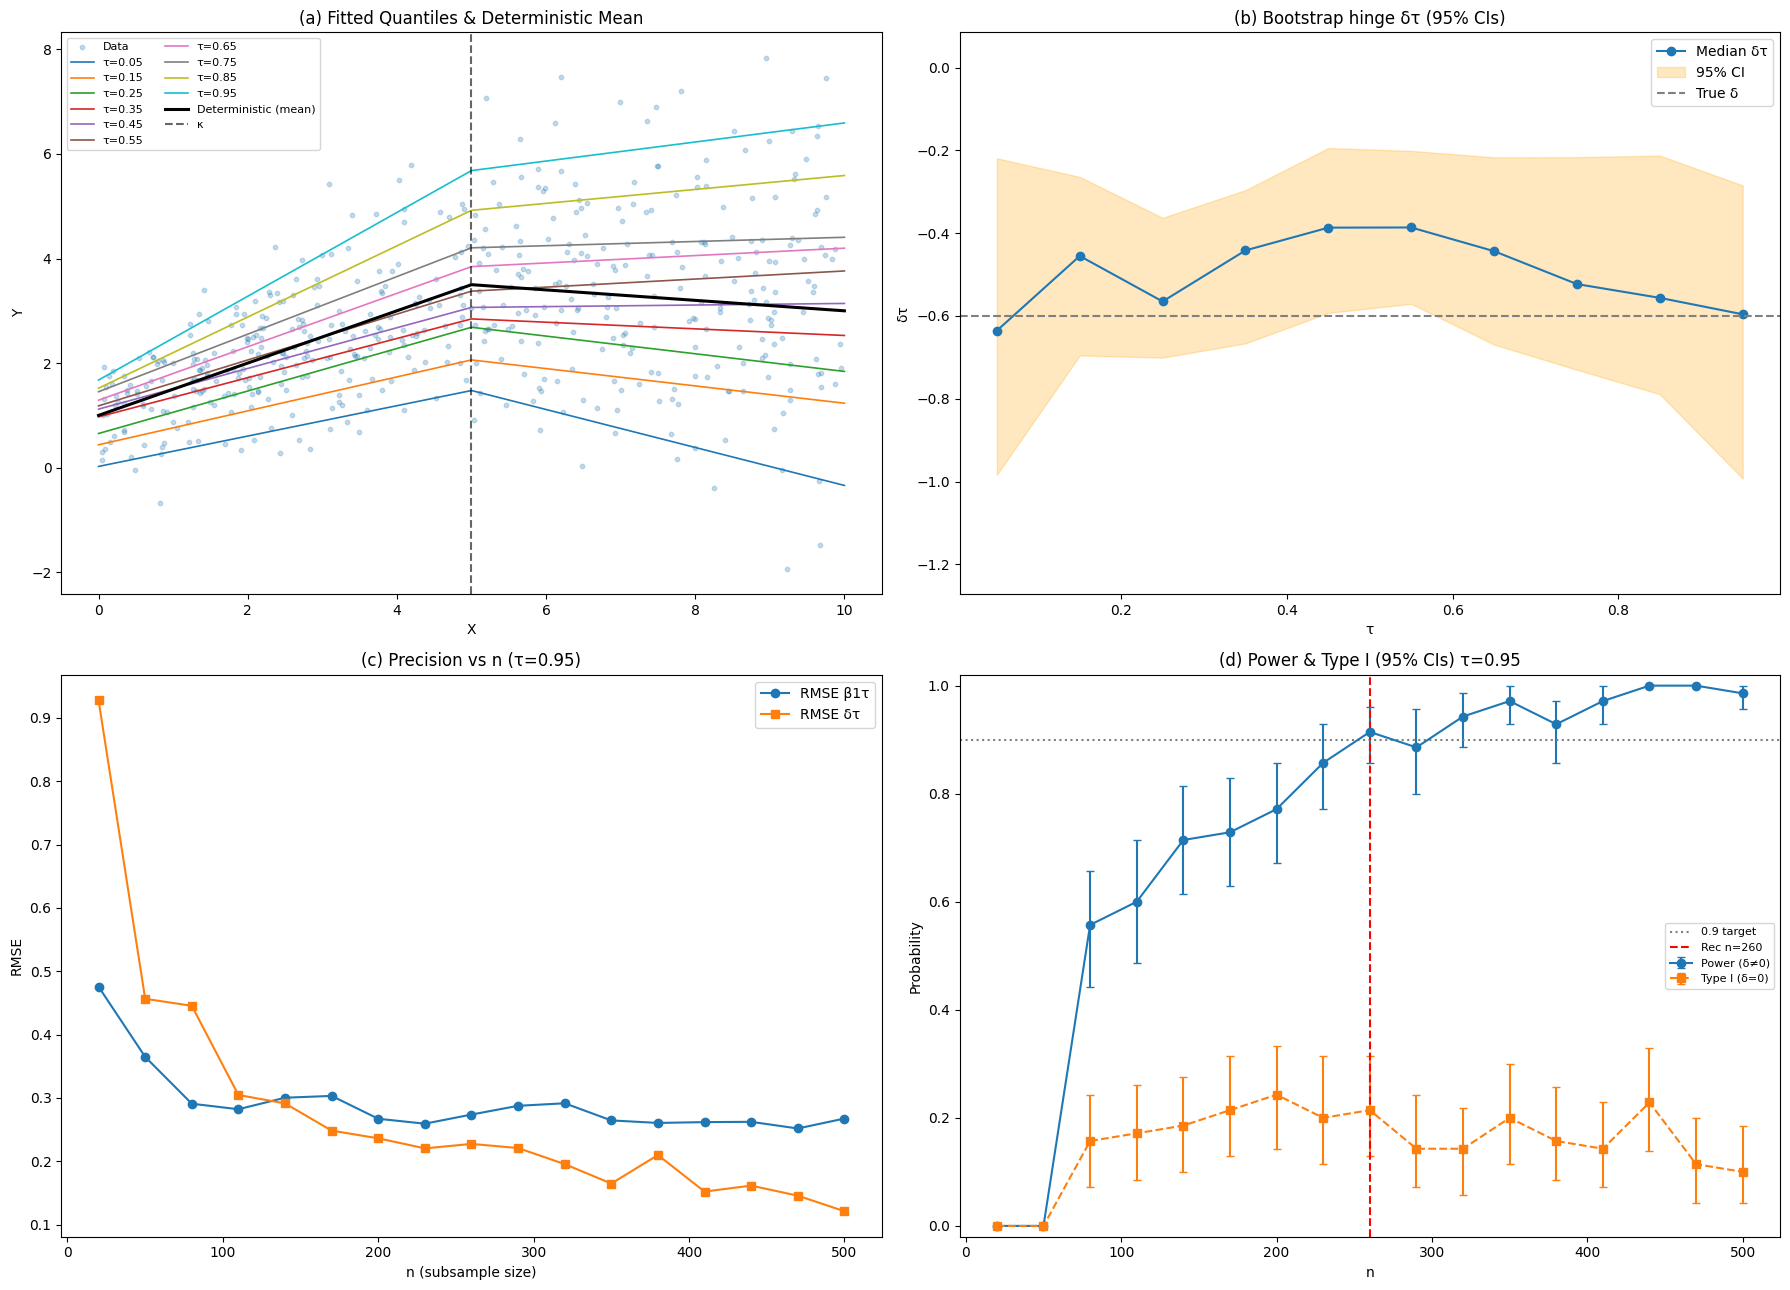
\includegraphics[width=0.9\textwidth]{../results/preliminary_results/power_sensitivity_evaluation_test.png}
\caption{Power and Sensitivity Analysis on Quantile Regression with Simulated Data, showing the impact of sample size and noise level on the detection of significant quantile regression coefficients.}
\label{fig:power_sensitivity_analysis_simulation}
\end{figure}
